\documentclass{article}
\usepackage{graphicx} 
\usepackage{float}
\usepackage{booktabs}
\usepackage{array}
\usepackage{arydshln}
\usepackage{siunitx}
\usepackage{hyperref}
\usepackage{cancel}
\usepackage{changepage}
\usepackage{placeins}
\usepackage{enumitem}

%\usepackage{showframe}
%\usepackage{times}

\usepackage{tabularx}
\usepackage{amsmath, amssymb, amscd, MnSymbol, mathrsfs}
\usepackage{cellspace}
\usepackage{tikz}
\usetikzlibrary{calc, patterns, angles, quotes, decorations.markings, decorations.pathmorphing, hobby}
\usepackage{xfrac}

\usepackage{chemfig}
\usepackage{caption}
\usepackage{tcolorbox}
\usepackage{bm}
\usepackage{pdfpages}
\usepackage{empheq}
\usepackage{pgfplots}
\pgfplotsset{compat=1.18}
\usepackage[oldvoltagedirection]{circuitikz}
\usepackage{microtype}
\usepackage{tikz-3dplot}
\usepackage{bibref}
\usepackage{textcomp}
% Custom commands
\newcommand{\vect}[1]{\boldsymbol{\mathbf{#1}}}
\newcolumntype{C}{>{\centering\arraybackslash}X}
\newcolumntype{M}[1]{>{\centering\arraybackslash}m{#1}}

\usetikzlibrary{external}
\tikzexternalize[prefix=figures/]

\newcommand\myfrac[2]{\sfrac{#1\mkern-1.2mu}{#2}}
\usepackage{xcolor}

% Define custom colors
\definecolor{darkblue}{rgb}{0.1,0.1,0.5} % A dark blue shade
\definecolor{formalshade}{rgb}{0.95,0.95,1} % A light blue shade for the background

% For the adjustwidth environment
\PassOptionsToPackage{strict}{changepage}
\usepackage{changepage}

% For formal definitions
\usepackage{framed}

\newcommand{\formalsource}{} % Initialize an empty macro to store the source text

\newenvironment{formal}[1][]{% Start of the environment
    \renewcommand{\formalsource}{#1}% Store the optional argument
    \def\FrameCommand{%
        \hspace{1pt}%
        {\color{darkblue}\vrule width 2pt}%
        {\color{formalshade}\vrule width 4pt}%
        \colorbox{formalshade}%
    }%
    \MakeFramed{\advance\hsize-\width\FrameRestore}%
    \noindent\hspace{-4.55pt}% Disable indenting the first paragraph
    \begin{adjustwidth}{}{7pt}%
        \vspace{2pt}%
    }%
    {%
        \vspace{2pt}%
        \ifx\formalsource\empty % Check if the source is empty
        \else
        \hfill{\footnotesize{\formalsource}}% Align source to the bottom-right
        \fi
    \end{adjustwidth}\endMakeFramed%
}


% Custom itemize list with images for positive and negative items
\newlist{gitemize}{itemize}{1} % Just one level for the list
\setlist[gitemize,1]{
    leftmargin=2.8em, % Adjust the margin for the list
    labelsep=1em % Control the space between the label and the list item
}

% Define checkmark and cross symbols for positive and negative items
\newcommand{\checkitem}{\raisebox{-0.25\height}{\includegraphics[width=0.4cm]{checkmark.png}}}
\newcommand{\crossitem}{\raisebox{-0.25\height}{\includegraphics[width=0.4cm]{cross.png}}}


\usepackage[margin=1in, left=0.8in, right=0.8in, includeheadfoot]{geometry}
\usepackage{fancyhdr}
\usepackage{graphicx}
\usepackage{tabularray}
\usepackage{varwidth} 


\pagestyle{fancy}
\fancyhf{}


\renewcommand{\headrulewidth}{0.4pt}
\renewcommand{\footrulewidth}{0.4pt}

\fancyhead[L]{
\includegraphics[height=1.2cm]{images/Kingston_University_London_logo_200-tablet.png}}
\fancyhead[R]{EG4019 - ME - Engineering Mechanics and Materials}
\fancyfoot[C]{Department of Mechanical Engineering}
\fancyfoot[R]{\thepage}

\geometry{top=0.5in,bottom=0.69in}
\usepackage{scalerel}

\setlength{\headheight}{30pt}
\setlength{\footskip}{20pt}


\usepackage[export]{adjustbox}
\usepackage{tocloft}
\renewcommand{\cfttoctitlefont}{}
\renewcommand{\contentsname}{}
\renewcommand{\cftsecleader}{\cftdotfill{\cftdotsep}}

\setlength{\cftbeforesecskip}{0.5em}


\usepackage{xurl}

\renewcommand{\theequation}{\text{Eq.}~\arabic{equation}}
%Refer to the equation as \eqref{equation}.
\usepackage{caption}  % This package allows captioning outside of a float


\usetikzlibrary{patterns}

\usetikzlibrary{patterns.meta}

\pgfdeclarepattern{
    name=hatch,
    parameters={\hatchsize,\hatchangle,\hatchlinewidth},
    bottom left={\pgfpoint{-.1pt}{-.1pt}},
    top right={\pgfpoint{\hatchsize+.1pt}{\hatchsize+.1pt}},
    tile size={\pgfpoint{\hatchsize}{\hatchsize}},
    tile transformation={\pgftransformrotate{\hatchangle}},
    code={
        \pgfsetlinewidth{\hatchlinewidth}
        \pgfpathmoveto{\pgfpoint{-.1pt}{-.1pt}}
        \pgfpathlineto{\pgfpoint{\hatchsize+.1pt}{\hatchsize+.1pt}}
        \pgfpathmoveto{\pgfpoint{-.1pt}{\hatchsize+.1pt}}
        \pgfpathlineto{\pgfpoint{\hatchsize+.1pt}{-.1pt}}
        \pgfusepath{stroke}
    }
}

\tikzset{
    hatch size/.store in=\hatchsize,
    hatch angle/.store in=\hatchangle,
    hatch line width/.store in=\hatchlinewidth,
    hatch size=5pt,           % Smaller hatch size for fewer lines
    hatch angle=45pt,         % More angle to spread lines
    hatch line width=.5pt,    % Thin lines
}




\begin{document}
        

    \vspace*{\fill}
    \begin{center}
        \textbf{\Huge Laboratory Report}\\[10pt]
        \LARGE \textbf{Tensile Test}
    \end{center}
    \vspace*{\fill}

    \Large    
    \begin{tabular}{@{}l l l@{}}
        \textbf{Submitted by:} & Sakariye Abiikar (Group Leader)\phantom{ssssss} & K2371673 \\
        & Sandeep Singh & K2314795 \\
        & Aland Floyd Noronha & K2423819 \\
        & Alan Roy & K2314478 \\
        & Judas Surname & K5671234 \\
    \end{tabular}
    
    \vspace*{\fill}
    
    \begin{tabular}{@{}l l@{}}
        \textbf{Key Dates:} & Date of practical: \\
        & Deadline: 31/12/2024 \\
        & Date of submission: \\
    \end{tabular}
    \vspace*{\fill}
    
    \large
    \newpage\noindent\vspace{2em}
    \begin{center}
        \LARGE \textbf{Contribution Table}\\[3em]
    \end{center}
    

    
    \begin{tblr}{
            colspec={Q[4cm]Q[4cm]Q[4cm]Q[3cm]},
            hlines,vlines,
            cells={valign=m,halign=c},
            rows={ht=4\baselineskip},
            row{1}={ht=1.5\baselineskip,font=\bfseries},
        }
        Student & Course & Contribution & Picture \\ 
        Sakariye Abiikar & Mechanical Engineering & Results, Theory, Recommendations & 
\includegraphics[width=2cm,valign=c]{images/profile.jpg} \\ 
        Andrew Surname & Aviation & Introduction & 
\includegraphics[width=2cm,valign=c]{images/profile.jpg} \\ 
        Lucas Surname & Astro & Results & 
\includegraphics[width=2cm,valign=c]{images/profile.jpg} \\ 
        James Surname & Mechanical Engineering & Discussion, References & 
\includegraphics[width=2cm,valign=c]{images/profile.jpg} \\ 
        Judas Surname & Civil Engineering &  & 
\includegraphics[width=2cm,valign=c]{images/profile.jpg} \\ 
    \end{tblr}
    
    \normalsize
    \newpage\noindent\vspace{1em}
    \begin{center}
        \LARGE \textbf{Table of Contents}\\[1.5em]
    \end{center}
    \tableofcontents
    \thispagestyle{fancy}


    \large\newpage\vspace*{-20pt}

    \section{Abstract}
    \vspace*{1em}
    This study investigated the effects of two thermal treatments on the mechanical properties of HE30/BS1476 aluminium alloy, initially characterized by a hardness of 120 HV5, an elastic modulus of 6 GPa, and an ultimate tensile strength of 500 MPa. The alloy underwent two heat treatments: first, heating for 90 minutes at 520\textdegree C, followed by an additional 40 minutes at 184\textdegree C in open air. Three distinct alloy variations were produced as a result of these treatments. The aim of the research was to quantify changes in hardness, modulus of elasticity, yield strength, ultimate tensile strength (UTS), and percentage elongation. Hardness was measured using a Zwick Roell ZHU hardness testing machine with a 5 kg load (HV5) (See Appendix A), and properties such as stress and strain were derived from data obtained using a Zwick Roell 2050 tensile testing machine.
%   {Needs small info on results and reflection/conclusion (to be added at a later date)}
   
    
    \newpage\vspace*{-20pt}
\section{Introduction}

In engineering, the selection and optimization of materials significantly influence the performance of designs, particularly in the aerospace, automotive, and construction industries. Aluminium alloys are highly valued in these sectors due to their excellent strength-to-weight ratio and corrosion resistance, especially in applications requiring mechanical improvements through controlled processes (thyssenkrupp, 2023).\\[8pt]
Research by metallurgists such as Sorby and Sauveur has demonstrated that \textbf{heat treatment} can significantly enhance the properties of alloys. By altering the microstructure, heat treatments improve tensile strength, hardness, and elasticity. Techniques such as quenching and solution heat treatment are tailored to achieve specific mechanical properties based on the alloy’s intended application (Eurotherm, 2024).\\[8pt] 
\textbf{Aging} is a heat treatment process used to enhance the mechanical properties of aluminum alloys. It involves two main stages: first, the alloy is heated to dissolve alloying elements and then rapidly cooled, creating a supersaturated solid solution. Following this, the alloy undergoes artificial aging, where it is reheated to a lower temperature for a set period. This allows for the formation of fine particles that strengthen the material by impeding dislocation movement, thereby improving its hardness and tensile strength. Aging is crucial for optimizing the performance of aluminum alloys used in various applications (Rajaa et al., 2018).\\[8pt]
The significance of heat treatments is further supported by research. In one study, for example, the hardness of Al 6082 alloy increased from 65 BHN to 102 BHN after 8 hours of solution heat treatment. Furthermore, the alloy's tensile strength increased from 154 MPa to 280 MPa after being aged for 6 hours at 205\textdegree C and 495\textdegree C (Singh et al., 2023). Aluminium alloys like HE30 are ideal for demanding applications in the automotive and aerospace industries because of these microstructural improvements.\\[8pt]
This research investigates the response of HE30 aluminium alloy to thermal treatments, focusing on changes in its mechanical properties.

\newpage\vspace*{-20pt}
\section{Method}
This laboratory research primarily focused on evaluating the mechanical properties of our alloy samples, including key metrics such as yield strength, ultimate tensile strength (UTS), modulus of elasticity, hardness, and percentage elongation. These properties are essential for understanding the material's behavior under stress and assessing its suitability for various engineering applications.\\[8pt]
The methodologies employed in this study were designed to optimize the data obtained from individual experiments on the alloys' mechanical properties. By utilizing advanced data analysis techniques such as \textbf{Response Surface Methodology (RSM) and Fraction Factorial Design (FFD)} (See Appendix C), we uncovered correlations and dependencies that might otherwise remain hidden. For instance, tensile testing, beyond yielding basic parameters like UTS and modulus of elasticity, provided insights into failure mechanisms and material behavior under specific conditions. This approach reduces the need for extensive experimental operations while deepening our understanding of the alloys' properties and enabling predictive modeling. By focusing on a minimal set of tests that deliver insights into multiple material properties, the methodology ensures each procedure is maximally informative, minimizing resource usage and reducing the likelihood of error.\\[8pt]
Building on this optimized experimental design, the research approach utilized in this study incorporates an \textbf{Integrated Testing Strategy (ITS)}. ITS combines collected data to provide a comprehensive and precise assessment of the alloy's mechanical properties. It reduces redundancy and streamlines the evaluation process by avoiding reliance on a single test or series of tests. As an example of broader interdisciplinary efforts, the ITS developed in this study enhances experimental efficiency while minimizing costs and resource consumption (Rovida et al., 2015; Alan Turing Institute, 2024).\\[8pt]
Our approach was characterized by the following key components:
\begin{enumerate}[itemsep=-0.5mm]
    \item {Dimensional Analysis}
    \item {Hardness Testing}
    \item {Tensile Testing} 
    \item {Data analysis}
\end{enumerate}
Note that \textbf{Sample Preparation} is distinct from the testing process and is not considered part of the testing itself.\\[8pt]
By designing experiments that yield multiple insights from each procedure, we were able to conduct a thorough analysis of the alloy's mechanical properties while minimizing resource usage and potential sources of error. This method not only ensures the accuracy and reliability of our results but also provides a rich dataset for in-depth analysis and interpretation of the alloy's performance characteristics.
\newpage

\section{Experimental Procedures}
The alloys used in this study are derived from \textbf{HE30/BS1476}. The term \textbf{HE30} refers to a temper designation within the now-withdrawn \textbf{BS 1476} standard, which outlined heat treatment and aging processes for aluminium alloys. \textbf{BS 1476}, introduced in 1955 and revised until 1987, was officially withdrawn on June 21, 2022.\\[8pt]  
Though \textbf{BS 1476} is no longer active, its parameters for \textbf{HE30} remain linked to the aluminium alloy \textbf{6082}, a widely used material in engineering. While exact details from \textbf{BS 1476} are unavailable, \textbf{HE30} is consistently associated with 6082.  
\begin{itemize}[itemsep=-1mm]
    \item \textbf{T6} - Solution heat-treated and artificially aged.
    \item \textbf{O} - Soft.
    \item \textbf{T4} - Solution heat-treated and naturally aged.
    \item \textbf{T651} - Solution heat-treated, stress-relieved, and artificially aged.
\end{itemize}  
The absence of \textbf{BS 1476} does not impede the characterization of \textbf{HE30}. The chemical composition of \textbf{6082} is standardized under \textbf{EN 573-3}, aligning with widely recognized descriptions of the alloy.



\subsection{Description}
Key details are as follows:
\begin{formal}[Truventor, 2019]
Aluminium HE 30 alloy a.k.a AL 6082 is a medium strength alloy with excellent corrosion resistance. It
has the highest strength of 6000 (6XXX) series alloys. It is also known as a structural alloy. In block,
plate, or bar form, AL HE 30 alloy is most commonly used in machining.\\[8pt]
Although it is a relatively new alloy, due to its higher strength, AL HE 30 has replaced AL 6061 in many
applications. The addition of a large amount of manganese controls the grain structure which in turn
results in a stronger alloy.\\[8pt]
\begin{minipage}[t]{0.57\textwidth}
    \textbf{Characteristics:}
    \begin{itemize}[itemsep=-1mm]
    \item High strength-to-weight ratio makes it ideal for lightweight structures.
    \item Most versatile and highest strength alloy in the 6000 series Aluminum.
    \item Good machinability compared to metals like Stainless Steel (SS) and Mild Steel (MS).
    \item Lightweight and corrosion-resistant components.
    \item Alternative to plastics in high-stress applications.
    \item Lower fatigue strength and elastic strength compared to steels.
\end{itemize}
\end{minipage}\hspace{2.4em}
\begin{minipage}[t]{0.45\textwidth}
\textbf{Applications:}
\begin{itemize}[itemsep=-1mm]
    \item Automotive components.
    \item Electronic applications.
    \item Aerospace components.
    \item Trusses, frames, and beams.
\end{itemize}
\end{minipage}\\
\vspace{1pt}
\end{formal}
\newpage\noindent
While there may be minor differences in composition and performance between HE30, as defined by BS 1476, and the 6082 alloy, obtaining precise specifications for HE30 in the context of BS 1476 would necessitate consultation with the British Standards Institution (BSI), especially since the standard was officially withdrawn in 2022. For the purposes of this study, HE30 shall be considered equivalent to the 6082 alloy. Although not an exact equivalent, this assumption will serve as the foundation for analysing its qualities and aiding further talks.
\subsection{Composition}
\centering
\begin{minipage}{0.44\textwidth}
    \centering
    \renewcommand{\arraystretch}{1.4}

        \begin{tabular}{|>{\normalsize\bfseries}l|>{\normalsize}c|}
            \hline
            \large \textbf{Chemical Element} & \textbf{\% Present} \\ \hline
            Aluminium (Al)            & Balance             \\ \hline
            Copper (Cu)               & 0.1 max        \\ \hline
            Magnesium (Mg)            & 0.6 - 1.2         \\ \hline
            Silicon (Si)              & 0.7 - 1.3         \\ \hline
            Iron (Fe)                 & 0.5 max         \\ \hline
            Manganese (Mn)            & 0.4 - 1         \\ \hline
            Zinc (Zn)                 & 0.2 max        \\ \hline
            Chromium (Cr)             & 0.25 max        \\ \hline
            Titanium (Ti)             & 0.1 max        \\ \hline
            Other (Each)              & 0.05 max        \\ \hline
            Others (Total)            & 0.15 max        \\ \hline
        \end{tabular}
        \captionof{table}{Chemical Composition of Alloy 6082 (BS EN 573-3:2009)}
        \label{tab:composition_6082}

        
    \vspace{1em}
    \begin{tabular}{|>{\normalsize\bfseries}l|>{\normalsize}c|}
        \hline
        \large\textbf{Chemical Element} & \large\textbf{\% Present} \\ \hline
        Aluminium (Al)            & Remainder         \\ \hline
        Copper (Cu)               & 0.1 max           \\ \hline
        Magnesium (Mg)            & 0.4 - 1.5         \\ \hline
        Silicon (Si)              & 0.6 - 1.3         \\ \hline
        Iron (Fe)                 & 0.6 max           \\ \hline
        Manganese (Mn)            & 0.4 - 1         \\ \hline
        Zinc (Zn)                 & 0.1 max           \\ \hline
        Chromium (Cr)             & 0.5 max           \\ \hline
        Titanium (Ti)             & 0.2 max           \\ \hline
    \end{tabular}
    \captionof{table}{Chemical Composition of HE30/BS1476 according to Dr. Santiago's Data}
    \label{tab:composition_he30}
\end{minipage}
\hfill
\begin{minipage}{0.53\textwidth}
    The composition of 6082 generally follows the typical values for 6082 aluminium alloy, as shown in Table \ref{tab:composition_6082}.\\[1em]
    Once again, I stress that there may be minor differences in the composition of HE30, especially in accordance with the BS 1476 specifications.\\[1em] 
    The values listed here are provided for reference, but the exact composition of the HE30 alloy should be verified for accurate work in our lab, as it may not align with typical web standards.
    \vspace{1em}\hrule\vspace{1em}
    Although I do have actual information regarding the "Aluminium alloy HE30 BS1476" from Dr. Santiago shown in Table \ref{tab:composition_he30}, it is important to note that this source lacks proper documentation, and its credibility remains uncertain.\\[1em]
    The BS1476 has been withdrawn and has not been explicitly updated or replaced, as I stated. It is still largely unreferenced and not widely recognised in the contemporary literature. However this data source contradicts to much of what is being currently pertaining to the standard.\\[1em]
    Although there are significant differences between the two sources in terms of composition, I have chosen to adopt Dr. Santiago's version for the purpose of this work. This decision is based on the fact that the table he provided reflects the information he, as my instructor, has shared with me. While I acknowledge the discrepancies and the lack of clear sourcing in his data, I consider it appropriate to proceed with his version for expediency, particularly as it aligns with the guidance he has given in our coursework.
\end{minipage}\\

\raggedright

\subsection{Heat Treatments and Alloy Conditions}
Each sample was treated under different conditions to evaluate the effect of heat treatment on its mechanical properties. The samples were provided in the typical bone-shaped form for tensile testing. The heat treatment conditions are as follows:
\begin{itemize}[itemsep=-1mm]
    \item \textbf{AR (As Received)}: The sample was used without any heat treatment, in its initial state as supplied.
    
    \item \textbf{ST (Solution Treatment)}: The sample was heated at 520\textdegree C for 90 minutes to dissolve precipitates, improving ductility. The exact quenching method is unspecified.
    
    \item \textbf{PH (Precipitation Hardening)}: The sample was first heated at 520\textdegree C for 90 minutes, followed by aging at 184\textdegree C for 40 minutes to enhance strength and hardness.
\end{itemize}
These treatments were applied to assess how they influence the alloy's mechanical properties.



% Here is the guidline/rules for this subsection
% Experimental procedures describe the precise, step-by-step actions required to carry out an experiment—such as specific instructions like "do this" or "do that"—ensuring repeatability and accuracy in obtaining results. These procedures are intended to allow any individual to physically replicate the experiment.

%SAMPLES: 
% Description of the alloy, Composition, CSA (mention dimensions are measured by a calliper), Nomenclature, Heat treatments, Picture before testing, etc

% HARDNESS: 
% Testing machine (pics), Procedure (pics)

% TENSILE TEST: 
% Machine (pics), Procedure (pics)


\def\imas{2.4cm}
\subsection{Equipment List}
\begin{table}[H]
    \centering
    \begin{tblr}{
            colspec = {Q[4cm] Q[4cm] Q[8cm]},
            hlines, vlines,
            rows={ht=4\baselineskip},
            cell{1-4,6}{1} = {font=\bfseries},
            cells = {valign=m,halign=c},
            column{3} = {valign=h,halign=l},
            row{1} = {ht=2\baselineskip,font=\bfseries,c,m},
        }
        \textbf{Equipment} & \textbf{Image} & \textbf{Reasoning} \\ 
        Digital Caliper & 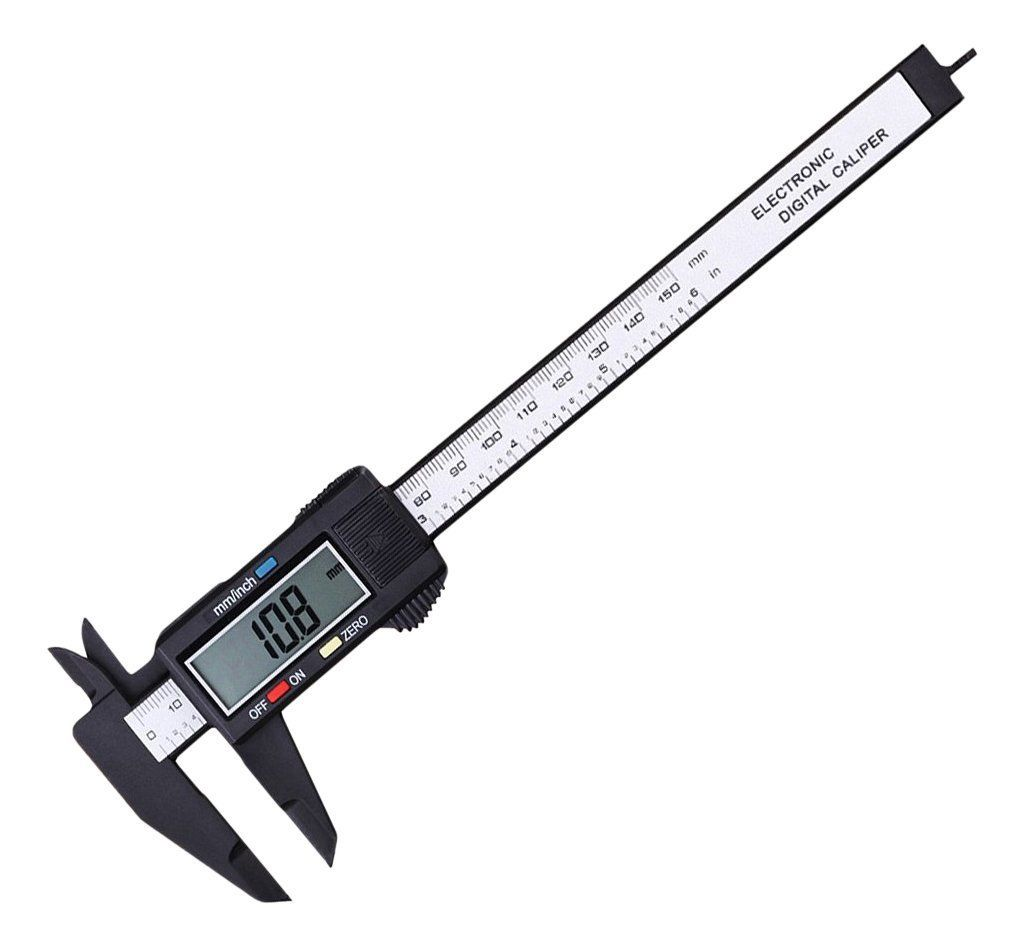
\includegraphics[width=\imas,valign=c]{images/digital_vernier_caliper.jpg} & Enables precise and accurate measurement of small dimensions, such as the diameter, thickness, and depth of samples, crucial for ensuring consistency in experimental setup and results. \\
        Vickers Hardness Testing Machine & 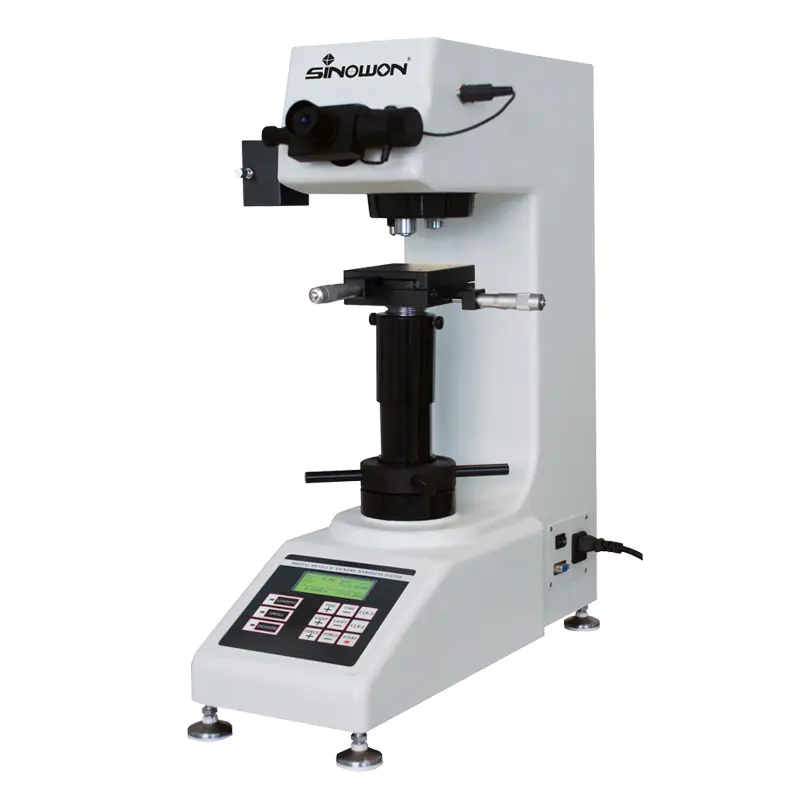
\includegraphics[width=\imas,valign=c]{images/hardness.png} & Used to assess the hardness of materials by applying a standardized force to create an indentation, which is then measured to determine the material's resistance to deformation. \\
        Zwick Roell 2050 Tensile Testing Machine & 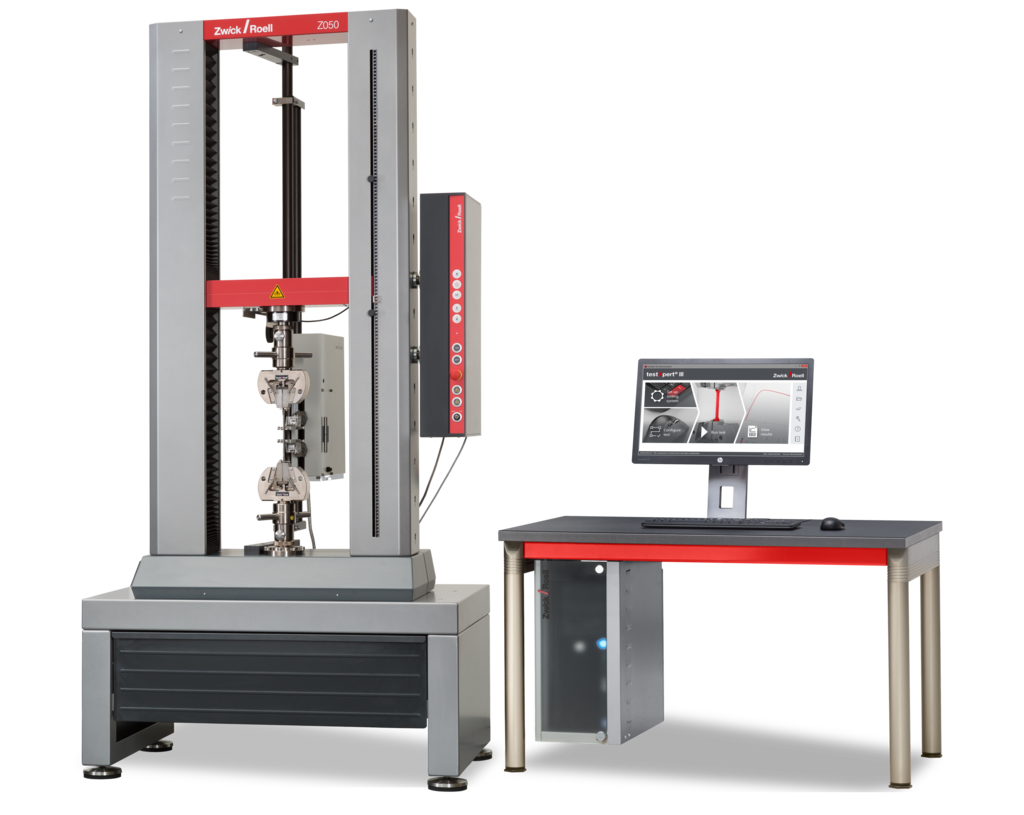
\includegraphics[width=\imas,valign=c]{images/tensilemachine.png} & Evaluates the tensile strength and mechanical properties of materials under uniaxial tension, providing data essential for material performance analysis and comparison. \\
        \textbf{Personal Protective Equipment (PPE):} Safety glasses, closed-toe shoes, lab coat & 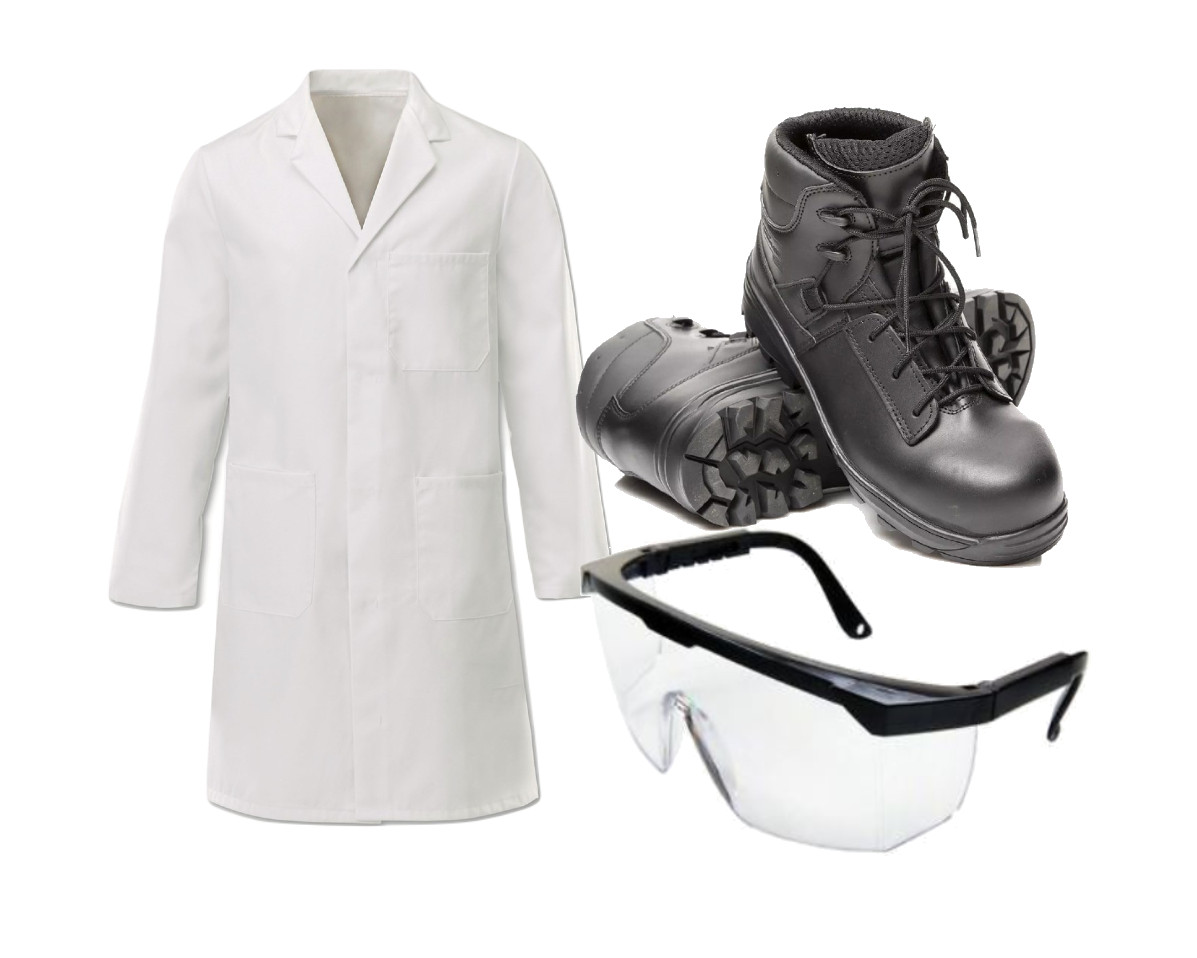
\includegraphics[width=\imas,valign=c]{images/ppe.jpg} & Protects against potential hazards in tensile testing, such as flying debris from specimen fracture, pinch points in the testing machine, and general laboratory risks further shown in Table \ref{tab:risk-assessment}.\\
        Camera/Smartphone and Stationery & 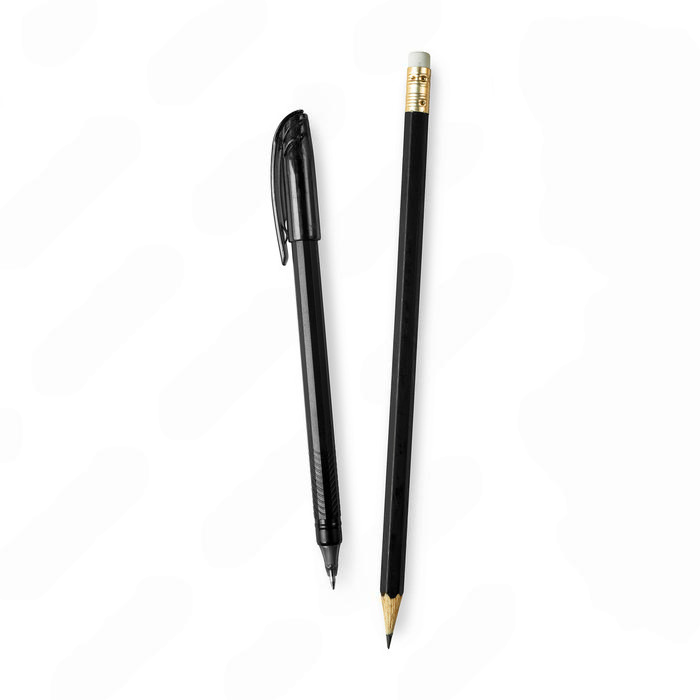
\includegraphics[width=\imas,valign=c]{images/stationary.png} & Essential for documenting experimental setups and procedures, capturing visual evidence of results, and recording detailed observations, calculations, and procedural notes for accurate reporting. \\
    \end{tblr}
    \caption{Overview of Equipment Used in the Experiment}
    \label{tab:equipment_overview}
\end{table}

    

\newcommand{\mr}[2]{%
    \begin{varwidth}{#2}%
        #1%
    \end{varwidth}%
}


\subsection{Risk Assessment}
The experimental procedures involved several potential hazards. The identified risks, their levels, and mitigation strategies are outlined below:
\begin{table}[h!]
    \centering
    \begin{tblr}{
            width=\linewidth,
            colspec={Q[4cm]Q[5cm]Q[2cm,c,m]Q[5cm]},
            rows = {ht=4\baselineskip},
            row{1} = {font=\bfseries,c,m,ht=1.5\baselineskip},            
            rows,columns = {valign=m},
            hlines, vlines
        }
        Hazard & Risk & Level of Risk & Control Measures \\
        \mr{Sharp edges of dogbone samples}{4cm} & \mr{Cuts or injuries while handling samples}{5cm} & Medium & \mr{Handle with care; use gloves when measuring and mounting samples.}{5cm} \\
        Tensile testing machine & \mr{Pinching or crushing injuries from moving parts}{5cm} & High & Keep hands and body away from moving components during operation; follow machine's safety protocols. \\
        \mr{Vickers hardness testing machine}{4cm} & Injury from improper handling or sample misplacement & Medium & Ensure proper training before operation; position samples correctly and keep fingers clear. \\
        \mr{General laboratory environment}{4cm} & Slips, trips, and falls due to clutter or spills & Low & Maintain a tidy workspace; clean spills immediately; wear appropriate footwear. \\
    \end{tblr}
    \caption{Identified hazards, associated risks, levels, and control measures.}
    \label{tab:risk-assessment}
\end{table}

\subsection{Conducting the Experiment}
For the experiment, we were provided with three samples, which are visually represented in the image below:
\begin{figure}[H] 
    \centering 
    \includegraphics[width=0.6\textwidth,height=0.3\textheight]{example-image} 
    \caption{Visual representation of the three samples} 
    \label{fig:samples} 
\end{figure}
\newpage\noindent
Additionally, we were given an A4 sheet with a form to complete, which looked as shown below:

\begin{figure}[H] 
    \centering 
    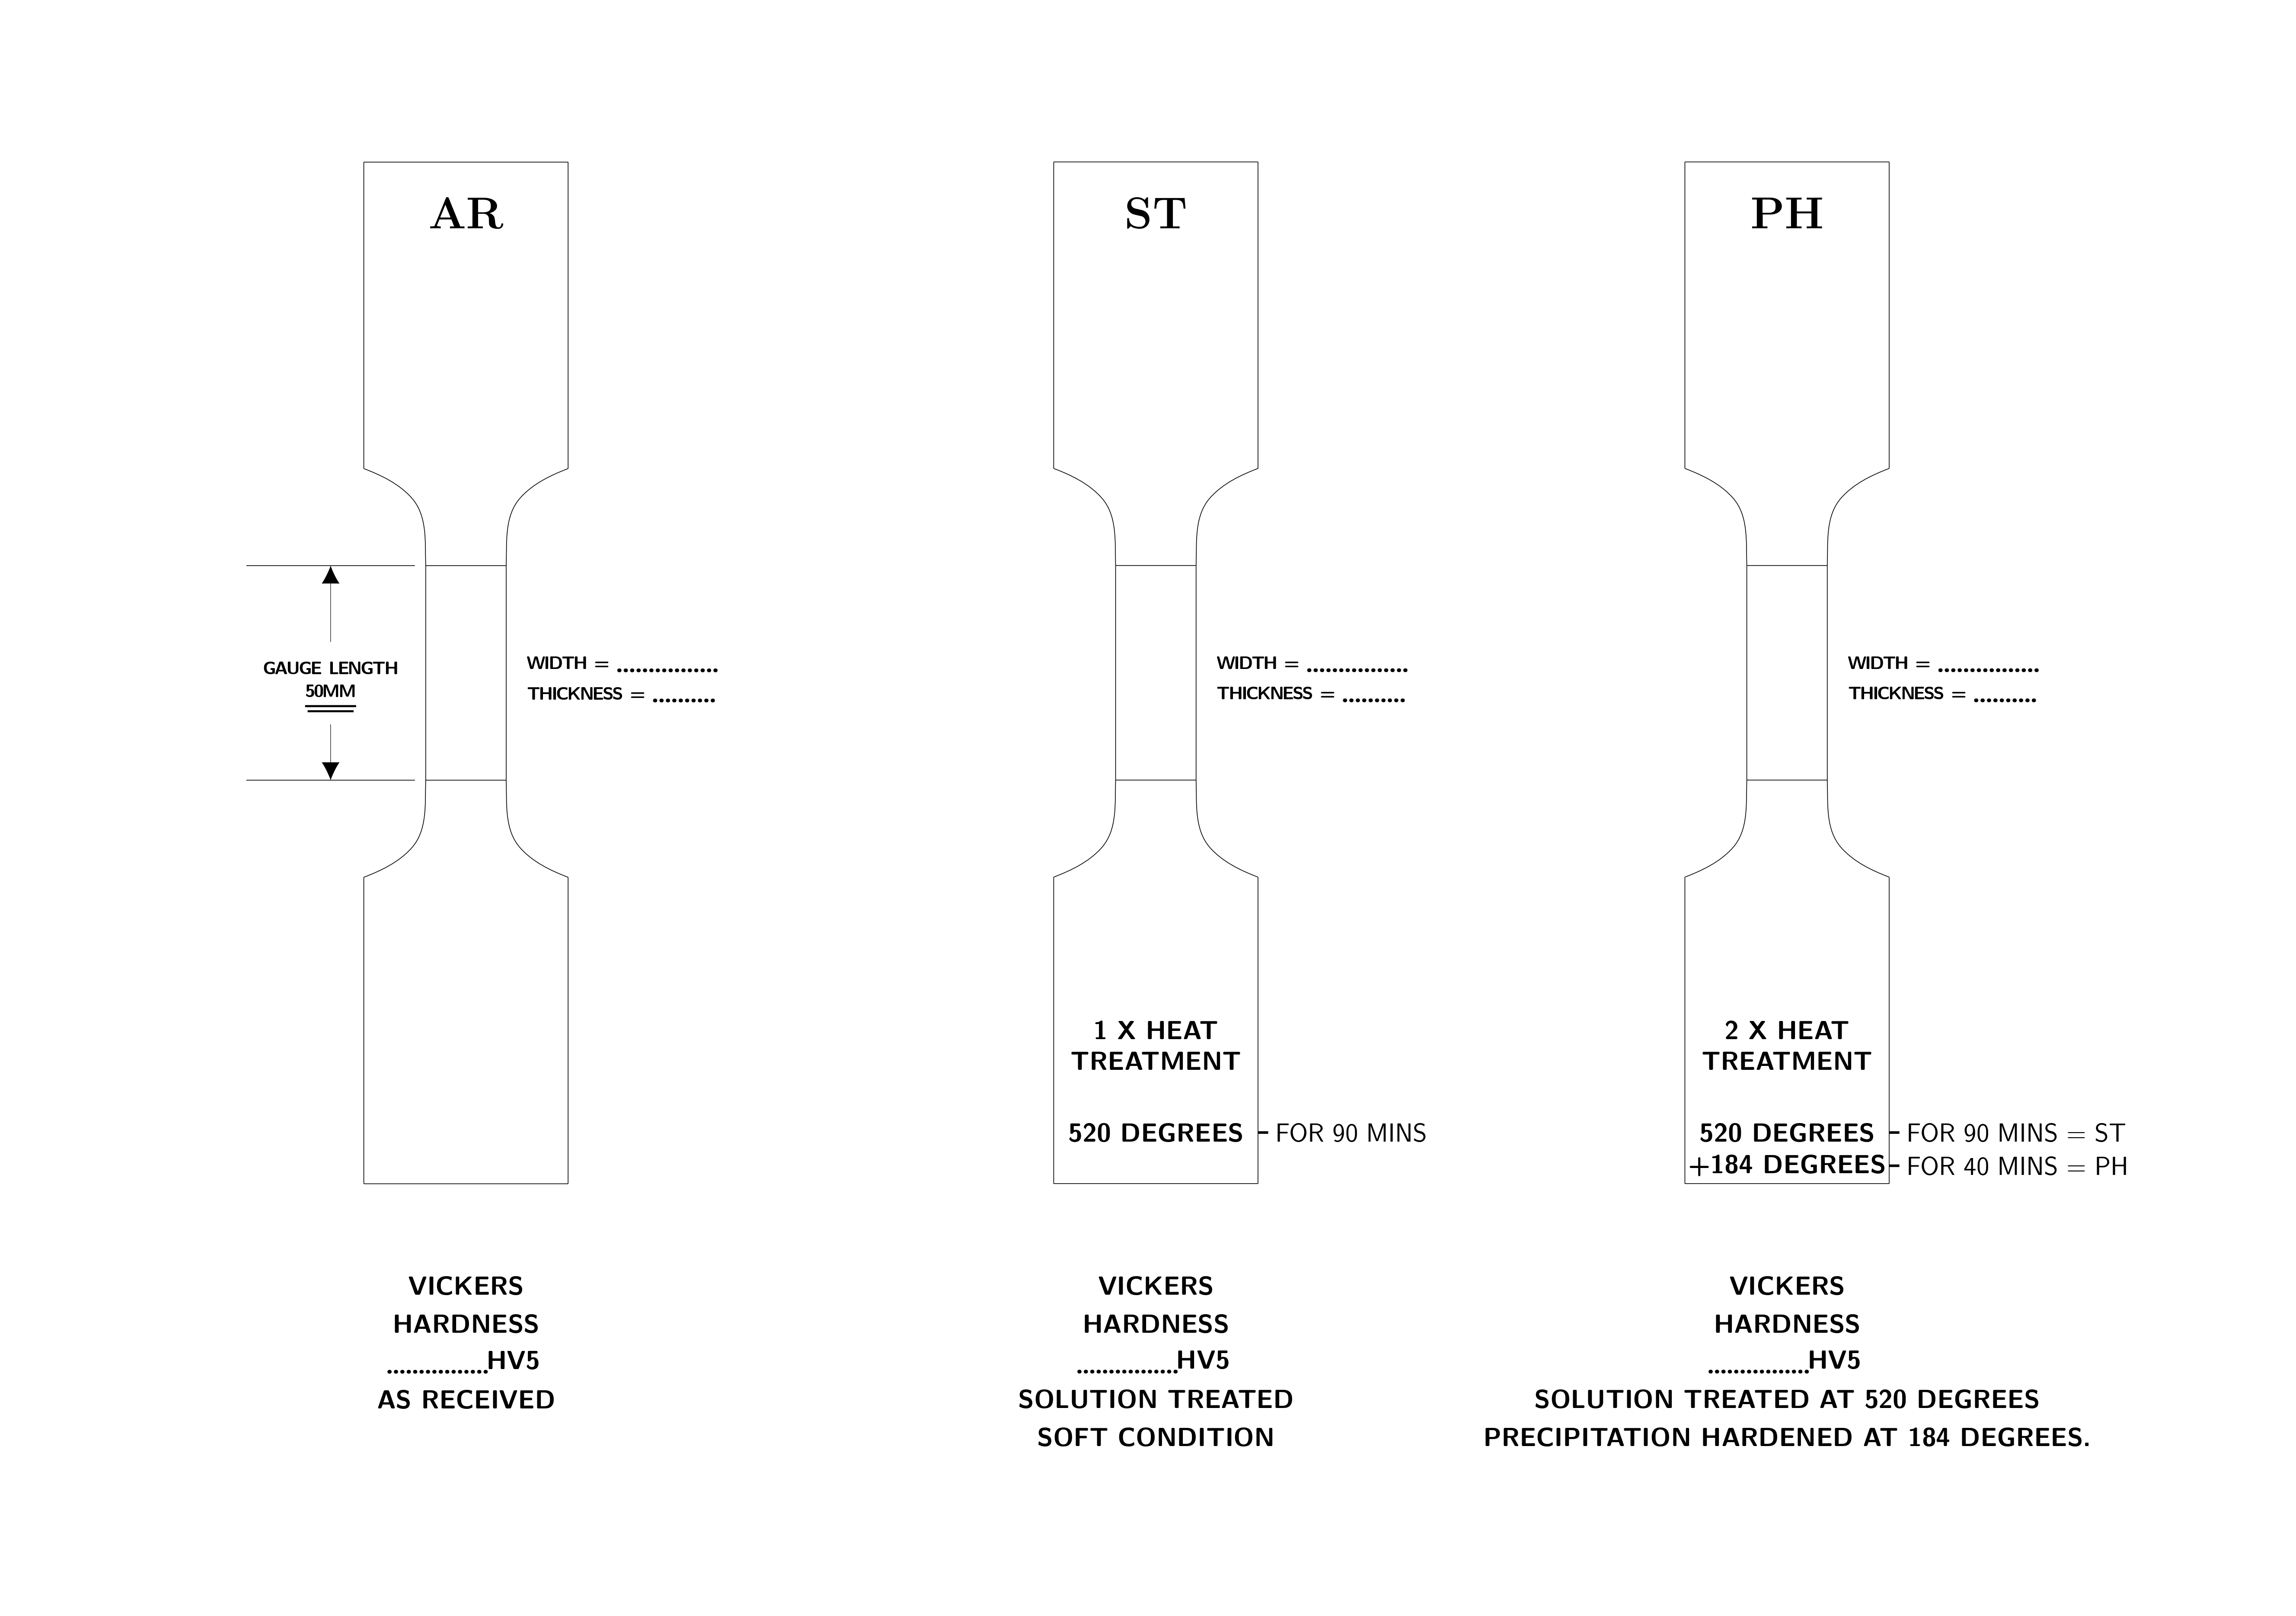
\includegraphics[width=\textwidth]{figures/alloys_base.jpg} 
    \caption{Form for recording sample measurements} 
    \label{fig:alloys} 
\end{figure}

On this form, we recorded the width, length (both in millimeters), and hardness (measured using the HV5 scale) for each of the three alloy samples as the initial phase of the experimental lab. These tasks were performed simultaneously, as they are relatively quick and do not require sequential completion. For instance, while the first sample was undergoing hardness testing, we measured the dimensions of the other samples.\\[8pt]
I will now demonstrate how we used digital calipers to measure the alloy samples in millimeters, along with the results obtained from these measurements:

\begin{minipage}{0.32\textwidth}
\begin{tikzpicture}[rotate around y=225, use Hobby shortcut,scale=0.35, every node/.style={scale=0.35}]
    \LARGE
    \def\width{4}
    \def\gap{10}
    \def\main{8}
    \def\curvy{1.9}
    \def\depth{3}
    
    \def\n{3.3}
    \def\z{1/\n}
    \pgfmathsetmacro{\s}{1-\z}
    
    \coordinate (A) at (0,\main,0);
    \coordinate (B) at (\width*\z-\width*\z*0.23,\main+\curvy-\curvy*0.7,0);
    \coordinate (C) at (\width*\z,\main+\curvy,0);
    
    \coordinate (A2) at (\width,\main,0);
    \coordinate (B2) at (\width*\s+\width*\z*0.23,\main+\curvy-\curvy*0.7,0);
    \coordinate (C2) at (\width*\s,\main+\curvy,0);
    
    \coordinate (A3) at (0,\main+\gap,0);
    \coordinate (B3) at (\width*\z-\width*\z*0.23,\main+\gap-\curvy+\curvy*0.7,0);
    \coordinate (C3) at (\width*\z,\main+\gap-\curvy,0);
    
    \coordinate (A4) at (\width,\main+\gap,0);
    \coordinate (B4) at (\width*\s+\width*\z*0.23,\main+\gap-\curvy+\curvy*0.7,0);
    \coordinate (C4) at (\width*\s,\main+\gap-\curvy,0);
    
    % Back variation with \depth (subtracting \depth from the z-coordinate)
    \coordinate (A') at (0,\main,\depth);
    \coordinate (B') at (\width*\z-\width*\z*0.23,\main+\curvy-\curvy*0.7,\depth);
    \coordinate (C') at (\width*\z,\main+\curvy,\depth);
    
    \coordinate (A2') at (\width,\main,\depth);
    \coordinate (B2') at (\width*\s+\width*\z*0.23,\main+\curvy-\curvy*0.7,\depth);
    \coordinate (C2') at (\width*\s,\main+\curvy,\depth);
    
    \coordinate (A3') at (0,\main+\gap,\depth);
    \coordinate (B3') at (\width*\z-\width*\z*0.23,\main+\gap-\curvy+\curvy*0.7,\depth);
    \coordinate (C3') at (\width*\z,\main+\gap-\curvy,\depth);
    
    \coordinate (A4') at (\width,\main+\gap,\depth);
    \coordinate (B4') at (\width*\s+\width*\z*0.23,\main+\gap-\curvy+\curvy*0.7,\depth);
    \coordinate (C4') at (\width*\s,\main+\gap-\curvy,\depth);
    
    
    % Back face fill
    \fill[black!40] 
    (0,0,\depth) -- (\width,0,\depth) -- (\width,\main,\depth) 
    to[hobby,tension=3] (\width,\main,\depth) .. (\width*\s+\width*\z*0.23,\main+\curvy-\curvy*0.7,\depth) .. (\width*\s,\main+\curvy,\depth) -- 
    (\width*\s,\main+\gap-\curvy,\depth) 
    to[hobby,tension=3] (\width*\s,\main+\gap-\curvy,\depth)  .. (\width*\s+\width*\z*0.23,\main+\gap-\curvy+\curvy*0.7,\depth) .. (\width,\main+\gap,\depth) --
    (\width,2*\main+\gap,\depth) -- (0,2*\main+\gap,\depth) -- 
    (0,\main+\gap,\depth) to[hobby,tension=3] (0,\main+\gap,\depth) .. (\width*\z-\width*\z*0.23,\main+\gap-\curvy+\curvy*0.7,\depth) .. (\width*\z,\main+\gap-\curvy,\depth) --
    (\width*\z,\main+\curvy,\depth) to[hobby,tension=3] (\width*\z,\main+\curvy,\depth) .. (\width*\z-\width*\z*0.23,\main+\curvy-\curvy*0.7,\depth) .. (0,\main,\depth) --
    cycle;
    
    % Curves fills with refined fades
    \fill[left color=gray!80, middle color=gray!50, right color=gray!20, opacity=0.8] 
    (A) to[hobby,tension=3] (A) .. (B) .. (C) -- (C3) to[hobby,tension=3] (C3) .. (B3) .. (A3) -- 
    (A3') to[hobby,tension=3] (A3') .. (B3') .. (C3') --
    (C') to[hobby,tension=3] (C') .. (B') .. (A') -- cycle;
    
    \fill[left color=gray!80, middle color=gray!50, right color=gray!20, opacity=0.8] 
    (A2) to[hobby,tension=3] (A2) .. (B2) .. (C2) -- (C4) to[hobby,tension=3] (C4) .. (B4) .. (A4) -- 
    (A4') to[hobby,tension=3] (A4') .. (B4') .. (C4') --
    (C2') to[hobby,tension=3] (C2') .. (B2') .. (A2') -- cycle;
    
    
    \draw[-,hobby,tension=3] (A2') .. (B2') .. (C2');
    \draw[-,hobby,tension=3] (A4') .. (B4') .. (C4');
    
    % Fill for bottom rectangle section
    \fill[black!33] 
    (0,0,0) -- (\width,0,0) -- (\width,0,\depth) -- (0,0,\depth) -- cycle;
    \fill[black!33] 
    (0,0,0) -- (0,\main,0) -- (0,\main,\depth) -- (0,0,\depth) -- cycle;
    \fill[black!40] 
    (\width,0,0) -- (\width,\main,0) -- (\width,\main,\depth) -- (\width,0,\depth) -- cycle;
    
    % Fill for top rectangle section
    \fill[black!30] 
    (0,2*\main+\gap,0) -- (\width,2*\main+\gap,0) -- (\width,2*\main+\gap,\depth) -- (0,2*\main+\gap,\depth) -- cycle;
    \fill[black!30] 
    (0,\main+\gap,0) -- (0,2*\main+\gap,0) -- (0,2*\main+\gap,\depth) -- (0,\main+\gap,\depth) -- cycle;
    \fill[black!33] 
    (\width,\main+\gap,0) -- (\width,2*\main+\gap,0) -- (\width,2*\main+\gap,\depth) -- (\width,\main+\gap,\depth) -- cycle;
    
    
    
    % Front face fill
    \fill[black!36] 
    (0,0,0) -- (\width,0,0) -- (\width,\main,0) 
    to[hobby,tension=3] (A2) .. (B2) .. (C2) -- 
    (\width*\s,\main+\gap-\curvy,0) 
    to[hobby,tension=3] (C4) .. (B4) .. (A4) --
    (\width,2*\main+\gap,0) -- (0,2*\main+\gap,0) -- 
    (0,\main+\gap,0) to[hobby,tension=3] (A3) .. (B3) .. (C3) --
    (\width*\z,\main+\curvy,0) to[hobby,tension=3] (C) .. (B) .. (A) --
    cycle;
    \draw[hobby,tension=3] (A) .. (B) .. (C);
    \draw[hobby,tension=3] (A2) .. (B2) .. (C2);
    \draw[hobby,tension=3] (A3) .. (B3) .. (C3);
    \draw[hobby,tension=3] (A4) .. (B4) .. (C4);
    \draw[dashed, opacity=0.3,hobby,tension=3] (A3') .. (B3') .. (C3');
    \draw[dashed, opacity=0.3,hobby,tension=3] (A') .. (B') .. (C');
    % Front face outline
    
    \draw[-] (0,0,0) -- (\width,0,0);
    \draw[-] (0,0,0) -- (0,\main,0);
    \draw[-] (\width*\z,\main+\curvy,0) -- (\width*\z,\main+\gap-\curvy,0);
    \draw[-] (0,\main+\gap,0) -- (0,2*\main+\gap,0);
    \draw[-] (0,2*\main+\gap,0) -- (\width,2*\main+\gap,0);
    \draw[-] (\width,2*\main+\gap,0) -- (\width,\main+\gap,0);
    \draw[-] (\width*\s,\main+\curvy,0) -- (\width*\s,\main+\gap-\curvy,0);    
    \draw[-] (\width,0,0) -- (\width,\main,0);
    
    
    
    
    
    % Back face outline
    
    
    \draw[dashed, opacity=0.3] (\width*\z,\main+\curvy,\depth) -- (\width*\z,\main+\gap-\curvy,\depth);
    \draw[-] (\width*\s,\main+\curvy,\depth) -- (\width*\s,\main+\gap-\curvy,\depth);
    \draw[dashed, opacity=0.3] (0,0,\depth) -- (\width,0,\depth);
    \draw[dashed, opacity=0.3] (0,0,\depth) -- (0,\main,\depth);
    \draw[-] (\width,0,\depth) -- (\width,\main,\depth);
    \draw[dashed, opacity=0.3] (0,\main+\gap,\depth) -- (0,2*\main+\gap,\depth);
    \draw[-] (0,2*\main+\gap,\depth) -- (\width,2*\main+\gap,\depth);
    \draw[-] (\width,2*\main+\gap,\depth) -- (\width,\main+\gap,\depth);
    
    
    
    % Connect front and back faces
    %botom
    \draw[-] (\width,\main,0) -- (\width,\main,\depth);
    \draw[-] (\width,0,0) -- (\width,0,\depth);
    \draw[dashed, opacity=0.3] (0,0,0) -- (0,0,\depth);
    \draw[-] (0,\main,0) -- (0,\main,\depth);
    %top
    \draw[-] (\width,\main+\gap,0) -- (\width,\main+\gap,\depth);
    \draw[-] (\width,2*\main+\gap,0) -- (\width,2*\main+\gap,\depth);
    \draw[-] (0,2*\main+\gap,0) -- (0,2*\main+\gap,\depth);
    \draw[dashed, opacity=0.3] (0,\main+\gap,0) -- (0,\main+\gap,\depth);
    
    
    
    %curves
    
    \draw[{Latex[length=1.93mm,width=1.93mm]}-{Latex[length=1.93mm,width=1.93mm]},line width=0.5mm] (C) -- (C2) node[below=-3,right=45] {\Huge \textbf{Width}};
    \draw[dashed, opacity=0.3] (C3) -- (C4);
    \draw[dashed, opacity=0.3] (C') -- (C2');
    \draw[dashed, opacity=0.3] (C3') -- (C4');
    \draw[dashed, opacity=0.3] (C) -- (C');
    \draw[{Latex[length=1.93mm,width=1.93mm]}-{Latex[length=1.93mm,width=1.93mm]},line width=0.5mm] (C2) -- (C2') node[below=-2,left] {\Huge \textbf{Thickness}};
    \draw[dashed, opacity=0.3] (C3) -- (C3');
    \draw[dashed, opacity=0.3] (C4) -- (C4');
    
    \draw[latex-latex, line width=0.5mm] 
    ($ (C) - (0.4,0,0) $) 
    -- ($ (C3) - (0.4,0,0) $) 
    node[right=5, midway] {\Huge \textbf{Length}};
    
\end{tikzpicture}
\end{minipage}\hfill
\begin{minipage}{0.65\textwidth}
\vspace{-1.5em}
\subsection{Measurements}
\vspace{0.5em}
\begin{center}
    \begin{tblr}{
        width=\textwidth,
        colspec={X[2,c]X[1,c]X[1,c]X[1,c]},
        hlines,vlines,
        rows={ht=1\baselineskip},
        row{1} = {ht=1\baselineskip,font=\bfseries,c,m},
        cells={valign=m,halign=c}
    }
    Property (mm) & AR & ST & PH \\
    Width   & 11.98 & 12.00 & 11.97 \\
    Thickness & 6.00  & 6.38  & 6.18  \\
    Length & 50.00 & 50.00 & 50.00 \\
\end{tblr}
\end{center}
\captionof{table}{Dimensions of AR, ST, and PH}
\label{tab:dimensions}
\vspace{1em}
\noindent
We measured the dimensions of each alloy using a digital calliper and recorded the results on an A4 sheet (See Figure \ref{fig:alloys}). We were informed that the gauge length was 50 mm, but we did not measure it ourselves. Although checking measurements is good practice, this analysis does not require it because the gauge length has no bearing on the cross-sectional area (CSA) computations further explained below.
\end{minipage}\\
\vspace{1em}
\hspace{-2em}
\begin{minipage}{0.4\textwidth}
\hspace{1em}\begin{minipage}{0.3\textwidth} 
\centering
\begin{tikzpicture}[rotate around y=225, use Hobby shortcut, scale=0.25, every node/.style={scale=0.25}]
    \large
    \def\width{4}
    \def\gap{10}
    \def\main{8}
    \def\curvy{1.9}
    \def\depth{3}
    
    \def\n{3.3}
    \def\z{1/\n}
    \pgfmathsetmacro{\s}{1-\z}
    
    \coordinate (A) at (0,\main,0);
    \coordinate (B) at (\width*\z-\width*\z*0.23,\main+\curvy-\curvy*0.7,0);
    \coordinate (C) at (\width*\z,\main+\curvy,0);
    
    \coordinate (A2) at (\width,\main,0);
    \coordinate (B2) at (\width*\s+\width*\z*0.23,\main+\curvy-\curvy*0.7,0);
    \coordinate (C2) at (\width*\s,\main+\curvy,0);
    
    \coordinate (A3) at (0,\main+\gap,0);
    \coordinate (B3) at (\width*\z-\width*\z*0.23,\main+\gap-\curvy+\curvy*0.7,0);
    \coordinate (C3) at (\width*\z,\main+\gap-\curvy,0);
    
    \coordinate (A4) at (\width,\main+\gap,0);
    \coordinate (B4) at (\width*\s+\width*\z*0.23,\main+\gap-\curvy+\curvy*0.7,0);
    \coordinate (C4) at (\width*\s,\main+\gap-\curvy,0);
    
    % Back variation with \depth (subtracting \depth from the z-coordinate)
    \coordinate (A') at (0,\main,\depth);
    \coordinate (B') at (\width*\z-\width*\z*0.23,\main+\curvy-\curvy*0.7,\depth);
    \coordinate (C') at (\width*\z,\main+\curvy,\depth);
    
    \coordinate (A2') at (\width,\main,\depth);
    \coordinate (B2') at (\width*\s+\width*\z*0.23,\main+\curvy-\curvy*0.7,\depth);
    \coordinate (C2') at (\width*\s,\main+\curvy,\depth);
    
    \coordinate (A3') at (0,\main+\gap,\depth);
    \coordinate (B3') at (\width*\z-\width*\z*0.23,\main+\gap-\curvy+\curvy*0.7,\depth);
    \coordinate (C3') at (\width*\z,\main+\gap-\curvy,\depth);
    
    \coordinate (A4') at (\width,\main+\gap,\depth);
    \coordinate (B4') at (\width*\s+\width*\z*0.23,\main+\gap-\curvy+\curvy*0.7,\depth);
    \coordinate (C4') at (\width*\s,\main+\gap-\curvy,\depth);
    
    
    % Back face fill
    \fill[black!40] 
    (0,0,\depth) -- (\width,0,\depth) -- (\width,\main,\depth) 
    to[hobby,tension=3] (\width,\main,\depth) .. (\width*\s+\width*\z*0.23,\main+\curvy-\curvy*0.7,\depth) .. (\width*\s,\main+\curvy,\depth) -- 
    (\width*\s,\main+\gap-\curvy,\depth) 
    to[hobby,tension=3] (\width*\s,\main+\gap-\curvy,\depth)  .. (\width*\s+\width*\z*0.23,\main+\gap-\curvy+\curvy*0.7,\depth) .. (\width,\main+\gap,\depth) --
    (\width,2*\main+\gap,\depth) -- (0,2*\main+\gap,\depth) -- 
    (0,\main+\gap,\depth) to[hobby,tension=3] (0,\main+\gap,\depth) .. (\width*\z-\width*\z*0.23,\main+\gap-\curvy+\curvy*0.7,\depth) .. (\width*\z,\main+\gap-\curvy,\depth) --
    (\width*\z,\main+\curvy,\depth) to[hobby,tension=3] (\width*\z,\main+\curvy,\depth) .. (\width*\z-\width*\z*0.23,\main+\curvy-\curvy*0.7,\depth) .. (0,\main,\depth) --
    cycle;
    
    % Curves fills with refined fades
    \fill[left color=gray!80, middle color=gray!50, right color=gray!20, opacity=0.8] 
    (A) to[hobby,tension=3] (A) .. (B) .. (C) -- (C3) to[hobby,tension=3] (C3) .. (B3) .. (A3) -- 
    (A3') to[hobby,tension=3] (A3') .. (B3') .. (C3') --
    (C') to[hobby,tension=3] (C') .. (B') .. (A') -- cycle;
    
    \fill[left color=gray!80, middle color=gray!50, right color=gray!20, opacity=0.8] 
    (A2) to[hobby,tension=3] (A2) .. (B2) .. (C2) -- (C4) to[hobby,tension=3] (C4) .. (B4) .. (A4) -- 
    (A4') to[hobby,tension=3] (A4') .. (B4') .. (C4') --
    (C2') to[hobby,tension=3] (C2') .. (B2') .. (A2') -- cycle;
    
    
    \draw[-,hobby,tension=3] (A2') .. (B2') .. (C2');
    \draw[-,hobby,tension=3] (A4') .. (B4') .. (C4');
    
    % Fill for bottom rectangle section
    \fill[black!33] 
    (0,0,0) -- (\width,0,0) -- (\width,0,\depth) -- (0,0,\depth) -- cycle;
    \fill[black!33] 
    (0,0,0) -- (0,\main,0) -- (0,\main,\depth) -- (0,0,\depth) -- cycle;
    \fill[black!40] 
    (\width,0,0) -- (\width,\main,0) -- (\width,\main,\depth) -- (\width,0,\depth) -- cycle;
    
    % Fill for top rectangle section
    \fill[black!30] 
    (0,2*\main+\gap,0) -- (\width,2*\main+\gap,0) -- (\width,2*\main+\gap,\depth) -- (0,2*\main+\gap,\depth) -- cycle;
    \fill[black!30] 
    (0,\main+\gap,0) -- (0,2*\main+\gap,0) -- (0,2*\main+\gap,\depth) -- (0,\main+\gap,\depth) -- cycle;
    \fill[black!33] 
    (\width,\main+\gap,0) -- (\width,2*\main+\gap,0) -- (\width,2*\main+\gap,\depth) -- (\width,\main+\gap,\depth) -- cycle;
    
    
    
    % Front face fill
    \fill[black!36] 
    (0,0,0) -- (\width,0,0) -- (\width,\main,0) 
    to[hobby,tension=3] (A2) .. (B2) .. (C2) -- 
    (\width*\s,\main+\gap-\curvy,0) 
    to[hobby,tension=3] (C4) .. (B4) .. (A4) --
    (\width,2*\main+\gap,0) -- (0,2*\main+\gap,0) -- 
    (0,\main+\gap,0) to[hobby,tension=3] (A3) .. (B3) .. (C3) --
    (\width*\z,\main+\curvy,0) to[hobby,tension=3] (C) .. (B) .. (A) --
    cycle;
    \draw[hobby,tension=3] (A) .. (B) .. (C);
    \draw[hobby,tension=3] (A2) .. (B2) .. (C2);
    \draw[hobby,tension=3] (A3) .. (B3) .. (C3);
    \draw[hobby,tension=3] (A4) .. (B4) .. (C4);
    \draw[dashed, opacity=0.3,hobby,tension=3] (A3') .. (B3') .. (C3');
    \draw[dashed, opacity=0.3,hobby,tension=3] (A') .. (B') .. (C');
    % Front face outline
    
    \draw[-] (0,0,0) -- (\width,0,0);
    \draw[-] (0,0,0) -- (0,\main,0);
    \draw[-] (\width*\z,\main+\curvy,0) -- (\width*\z,\main+\gap-\curvy,0);
    \draw[-] (0,\main+\gap,0) -- (0,2*\main+\gap,0);
    \draw[-] (0,2*\main+\gap,0) -- (\width,2*\main+\gap,0);
    \draw[-] (\width,2*\main+\gap,0) -- (\width,\main+\gap,0);
    \draw[-] (\width*\s,\main+\curvy,0) -- (\width*\s,\main+\gap-\curvy,0);    
    \draw[-] (\width,0,0) -- (\width,\main,0);
    
    
    
    
    
    % Back face outline
    
    
    \draw[dashed, opacity=0.3] (\width*\z,\main+\curvy,\depth) -- (\width*\z,\main+\gap-\curvy,\depth);
    \draw[-] (\width*\s,\main+\curvy,\depth) -- (\width*\s,\main+\gap-\curvy,\depth);
    \draw[dashed, opacity=0.3] (0,0,\depth) -- (\width,0,\depth);
    \draw[dashed, opacity=0.3] (0,0,\depth) -- (0,\main,\depth);
    \draw[-] (\width,0,\depth) -- (\width,\main,\depth);
    \draw[dashed, opacity=0.3] (0,\main+\gap,\depth) -- (0,2*\main+\gap,\depth);
    \draw[-] (0,2*\main+\gap,\depth) -- (\width,2*\main+\gap,\depth);
    \draw[-] (\width,2*\main+\gap,\depth) -- (\width,\main+\gap,\depth);
    
    
    
    % Connect front and back faces
    %botom
    \draw[-] (\width,\main,0) -- (\width,\main,\depth);
    \draw[-] (\width,0,0) -- (\width,0,\depth);
    \draw[dashed, opacity=0.3] (0,0,0) -- (0,0,\depth);
    \draw[-] (0,\main,0) -- (0,\main,\depth);
    %top
    \draw[-] (\width,\main+\gap,0) -- (\width,\main+\gap,\depth);
    \draw[-] (\width,2*\main+\gap,0) -- (\width,2*\main+\gap,\depth);
    \draw[-] (0,2*\main+\gap,0) -- (0,2*\main+\gap,\depth);
    \draw[dashed, opacity=0.3] (0,\main+\gap,0) -- (0,\main+\gap,\depth);
    
    
    
    %curves
    \draw[dashed, opacity=0.3] (C) -- (C2);
    \draw[dashed, opacity=0.3] (C3) -- (C4);
    \draw[dashed, opacity=0.3] (C') -- (C2');
    \draw[dashed, opacity=0.3] (C3') -- (C4');
    \draw[dashed, opacity=0.3] (C) -- (C');
    \draw[dashed, opacity=0.3] (C2) -- (C2');
    \draw[dashed, opacity=0.3] (C3) -- (C3');
    \draw[dashed, opacity=0.3] (C4) -- (C4');
    
    
    \fill[opacity=0.6,pattern={Lines[
        distance=1mm,
        angle=45,
        line width=0.4mm
        ]},
    pattern color=blue
    ] (C2) -- (C) -- (C3) -- (C4) -- cycle;

\end{tikzpicture}
\color{blue} \textbf{\textsf{CSA 1}}
\end{minipage}\hspace{-1em}
\begin{minipage}{0.3\textwidth}
    \centering
    \begin{tikzpicture}[rotate around y=225, use Hobby shortcut, scale=0.25, every node/.style={scale=0.25}]
        \large
        \def\width{4}
        \def\gap{10}
        \def\main{8}
        \def\curvy{1.9}
        \def\depth{3}
        
        \def\n{3.3}
        \def\z{1/\n}
        \pgfmathsetmacro{\s}{1-\z}
        
        \coordinate (A) at (0,\main,0);
        \coordinate (B) at (\width*\z-\width*\z*0.23,\main+\curvy-\curvy*0.7,0);
        \coordinate (C) at (\width*\z,\main+\curvy,0);
        
        \coordinate (A2) at (\width,\main,0);
        \coordinate (B2) at (\width*\s+\width*\z*0.23,\main+\curvy-\curvy*0.7,0);
        \coordinate (C2) at (\width*\s,\main+\curvy,0);
        
        \coordinate (A3) at (0,\main+\gap,0);
        \coordinate (B3) at (\width*\z-\width*\z*0.23,\main+\gap-\curvy+\curvy*0.7,0);
        \coordinate (C3) at (\width*\z,\main+\gap-\curvy,0);
        
        \coordinate (A4) at (\width,\main+\gap,0);
        \coordinate (B4) at (\width*\s+\width*\z*0.23,\main+\gap-\curvy+\curvy*0.7,0);
        \coordinate (C4) at (\width*\s,\main+\gap-\curvy,0);
        
        % Back variation with \depth (subtracting \depth from the z-coordinate)
        \coordinate (A') at (0,\main,\depth);
        \coordinate (B') at (\width*\z-\width*\z*0.23,\main+\curvy-\curvy*0.7,\depth);
        \coordinate (C') at (\width*\z,\main+\curvy,\depth);
        
        \coordinate (A2') at (\width,\main,\depth);
        \coordinate (B2') at (\width*\s+\width*\z*0.23,\main+\curvy-\curvy*0.7,\depth);
        \coordinate (C2') at (\width*\s,\main+\curvy,\depth);
        
        \coordinate (A3') at (0,\main+\gap,\depth);
        \coordinate (B3') at (\width*\z-\width*\z*0.23,\main+\gap-\curvy+\curvy*0.7,\depth);
        \coordinate (C3') at (\width*\z,\main+\gap-\curvy,\depth);
        
        \coordinate (A4') at (\width,\main+\gap,\depth);
        \coordinate (B4') at (\width*\s+\width*\z*0.23,\main+\gap-\curvy+\curvy*0.7,\depth);
        \coordinate (C4') at (\width*\s,\main+\gap-\curvy,\depth);
        
        
        % Back face fill
        \fill[black!40] 
        (0,0,\depth) -- (\width,0,\depth) -- (\width,\main,\depth) 
        to[hobby,tension=3] (\width,\main,\depth) .. (\width*\s+\width*\z*0.23,\main+\curvy-\curvy*0.7,\depth) .. (\width*\s,\main+\curvy,\depth) -- 
        (\width*\s,\main+\gap-\curvy,\depth) 
        to[hobby,tension=3] (\width*\s,\main+\gap-\curvy,\depth)  .. (\width*\s+\width*\z*0.23,\main+\gap-\curvy+\curvy*0.7,\depth) .. (\width,\main+\gap,\depth) --
        (\width,2*\main+\gap,\depth) -- (0,2*\main+\gap,\depth) -- 
        (0,\main+\gap,\depth) to[hobby,tension=3] (0,\main+\gap,\depth) .. (\width*\z-\width*\z*0.23,\main+\gap-\curvy+\curvy*0.7,\depth) .. (\width*\z,\main+\gap-\curvy,\depth) --
        (\width*\z,\main+\curvy,\depth) to[hobby,tension=3] (\width*\z,\main+\curvy,\depth) .. (\width*\z-\width*\z*0.23,\main+\curvy-\curvy*0.7,\depth) .. (0,\main,\depth) --
        cycle;
        
        % Curves fills with refined fades
        \fill[left color=gray!80, middle color=gray!50, right color=gray!20, opacity=0.8] 
        (A) to[hobby,tension=3] (A) .. (B) .. (C) -- (C3) to[hobby,tension=3] (C3) .. (B3) .. (A3) -- 
        (A3') to[hobby,tension=3] (A3') .. (B3') .. (C3') --
        (C') to[hobby,tension=3] (C') .. (B') .. (A') -- cycle;
        
        \fill[left color=gray!80, middle color=gray!50, right color=gray!20, opacity=0.8] 
        (A2) to[hobby,tension=3] (A2) .. (B2) .. (C2) -- (C4) to[hobby,tension=3] (C4) .. (B4) .. (A4) -- 
        (A4') to[hobby,tension=3] (A4') .. (B4') .. (C4') --
        (C2') to[hobby,tension=3] (C2') .. (B2') .. (A2') -- cycle;
        
        
        \draw[-,hobby,tension=3] (A2') .. (B2') .. (C2');
        \draw[-,hobby,tension=3] (A4') .. (B4') .. (C4');
        
        % Fill for bottom rectangle section
        \fill[black!33] 
        (0,0,0) -- (\width,0,0) -- (\width,0,\depth) -- (0,0,\depth) -- cycle;
        \fill[black!33] 
        (0,0,0) -- (0,\main,0) -- (0,\main,\depth) -- (0,0,\depth) -- cycle;
        \fill[black!40] 
        (\width,0,0) -- (\width,\main,0) -- (\width,\main,\depth) -- (\width,0,\depth) -- cycle;
        
        % Fill for top rectangle section
        \fill[black!30] 
        (0,2*\main+\gap,0) -- (\width,2*\main+\gap,0) -- (\width,2*\main+\gap,\depth) -- (0,2*\main+\gap,\depth) -- cycle;
        \fill[black!30] 
        (0,\main+\gap,0) -- (0,2*\main+\gap,0) -- (0,2*\main+\gap,\depth) -- (0,\main+\gap,\depth) -- cycle;
        \fill[black!33] 
        (\width,\main+\gap,0) -- (\width,2*\main+\gap,0) -- (\width,2*\main+\gap,\depth) -- (\width,\main+\gap,\depth) -- cycle;
        
        
        
        % Front face fill
        \fill[black!36] 
        (0,0,0) -- (\width,0,0) -- (\width,\main,0) 
        to[hobby,tension=3] (A2) .. (B2) .. (C2) -- 
        (\width*\s,\main+\gap-\curvy,0) 
        to[hobby,tension=3] (C4) .. (B4) .. (A4) --
        (\width,2*\main+\gap,0) -- (0,2*\main+\gap,0) -- 
        (0,\main+\gap,0) to[hobby,tension=3] (A3) .. (B3) .. (C3) --
        (\width*\z,\main+\curvy,0) to[hobby,tension=3] (C) .. (B) .. (A) --
        cycle;
        \draw[hobby,tension=3] (A) .. (B) .. (C);
        \draw[hobby,tension=3] (A2) .. (B2) .. (C2);
        \draw[hobby,tension=3] (A3) .. (B3) .. (C3);
        \draw[hobby,tension=3] (A4) .. (B4) .. (C4);
        \draw[dashed, opacity=0.3,hobby,tension=3] (A3') .. (B3') .. (C3');
        \draw[dashed, opacity=0.3,hobby,tension=3] (A') .. (B') .. (C');
        % Front face outline
        
        \draw[-] (0,0,0) -- (\width,0,0);
        \draw[-] (0,0,0) -- (0,\main,0);
        \draw[-] (\width*\z,\main+\curvy,0) -- (\width*\z,\main+\gap-\curvy,0);
        \draw[-] (0,\main+\gap,0) -- (0,2*\main+\gap,0);
        \draw[-] (0,2*\main+\gap,0) -- (\width,2*\main+\gap,0);
        \draw[-] (\width,2*\main+\gap,0) -- (\width,\main+\gap,0);
        \draw[-] (\width*\s,\main+\curvy,0) -- (\width*\s,\main+\gap-\curvy,0);    
        \draw[-] (\width,0,0) -- (\width,\main,0);
        
        
        
        
        
        % Back face outline
        
        
        \draw[dashed, opacity=0.3] (\width*\z,\main+\curvy,\depth) -- (\width*\z,\main+\gap-\curvy,\depth);
        \draw[-] (\width*\s,\main+\curvy,\depth) -- (\width*\s,\main+\gap-\curvy,\depth);
        \draw[dashed, opacity=0.3] (0,0,\depth) -- (\width,0,\depth);
        \draw[dashed, opacity=0.3] (0,0,\depth) -- (0,\main,\depth);
        \draw[-] (\width,0,\depth) -- (\width,\main,\depth);
        \draw[dashed, opacity=0.3] (0,\main+\gap,\depth) -- (0,2*\main+\gap,\depth);
        \draw[-] (0,2*\main+\gap,\depth) -- (\width,2*\main+\gap,\depth);
        \draw[-] (\width,2*\main+\gap,\depth) -- (\width,\main+\gap,\depth);
        
        
        
        % Connect front and back faces
        %botom
        \draw[-] (\width,\main,0) -- (\width,\main,\depth);
        \draw[-] (\width,0,0) -- (\width,0,\depth);
        \draw[dashed, opacity=0.3] (0,0,0) -- (0,0,\depth);
        \draw[-] (0,\main,0) -- (0,\main,\depth);
        %top
        \draw[-] (\width,\main+\gap,0) -- (\width,\main+\gap,\depth);
        \draw[-] (\width,2*\main+\gap,0) -- (\width,2*\main+\gap,\depth);
        \draw[-] (0,2*\main+\gap,0) -- (0,2*\main+\gap,\depth);
        \draw[dashed, opacity=0.3] (0,\main+\gap,0) -- (0,\main+\gap,\depth);
        
        
        
        %curves
        \draw[dashed, opacity=0.3] (C) -- (C2);
        \draw[dashed, opacity=0.3] (C3) -- (C4);
        \draw[dashed, opacity=0.3] (C') -- (C2');
        \draw[dashed, opacity=0.3] (C3') -- (C4');
        \draw[dashed, opacity=0.3] (C) -- (C');
        \draw[dashed, opacity=0.3] (C2) -- (C2');
        \draw[dashed, opacity=0.3] (C3) -- (C3');
        \draw[dashed, opacity=0.3] (C4) -- (C4');
        
        
        \fill[opacity=0.6,pattern={Lines[
            distance=1mm,
            angle=45,
            line width=0.4mm
            ]},
        pattern color=green!70!black
        ] (C2) -- (C4) -- (C4') -- (C2') -- cycle;
    \end{tikzpicture}    
    \color{green!50!black} \textbf{\textsf{CSA 2}}
\end{minipage}\hspace{-1em}
\begin{minipage}{0.3\textwidth}
    \centering
    \begin{tikzpicture}[rotate around y=225, use Hobby shortcut, scale=0.25, every node/.style={scale=0.25}]
    \large
    \def\width{4}
    \def\gap{10}
    \def\main{8}
    \def\curvy{1.9}
    \def\depth{3}
    
    \def\n{3.3}
    \def\z{1/\n}
    \pgfmathsetmacro{\s}{1-\z}
    
    \coordinate (A) at (0,\main,0);
    \coordinate (B) at (\width*\z-\width*\z*0.23,\main+\curvy-\curvy*0.7,0);
    \coordinate (C) at (\width*\z,\main+\curvy,0);
    
    \coordinate (A2) at (\width,\main,0);
    \coordinate (B2) at (\width*\s+\width*\z*0.23,\main+\curvy-\curvy*0.7,0);
    \coordinate (C2) at (\width*\s,\main+\curvy,0);
    
    \coordinate (A3) at (0,\main+\gap,0);
    \coordinate (B3) at (\width*\z-\width*\z*0.23,\main+\gap-\curvy+\curvy*0.7,0);
    \coordinate (C3) at (\width*\z,\main+\gap-\curvy,0);
    
    \coordinate (A4) at (\width,\main+\gap,0);
    \coordinate (B4) at (\width*\s+\width*\z*0.23,\main+\gap-\curvy+\curvy*0.7,0);
    \coordinate (C4) at (\width*\s,\main+\gap-\curvy,0);
    
    % Back variation with \depth (subtracting \depth from the z-coordinate)
    \coordinate (A') at (0,\main,\depth);
    \coordinate (B') at (\width*\z-\width*\z*0.23,\main+\curvy-\curvy*0.7,\depth);
    \coordinate (C') at (\width*\z,\main+\curvy,\depth);
    
    \coordinate (A2') at (\width,\main,\depth);
    \coordinate (B2') at (\width*\s+\width*\z*0.23,\main+\curvy-\curvy*0.7,\depth);
    \coordinate (C2') at (\width*\s,\main+\curvy,\depth);
    
    \coordinate (A3') at (0,\main+\gap,\depth);
    \coordinate (B3') at (\width*\z-\width*\z*0.23,\main+\gap-\curvy+\curvy*0.7,\depth);
    \coordinate (C3') at (\width*\z,\main+\gap-\curvy,\depth);
    
    \coordinate (A4') at (\width,\main+\gap,\depth);
    \coordinate (B4') at (\width*\s+\width*\z*0.23,\main+\gap-\curvy+\curvy*0.7,\depth);
    \coordinate (C4') at (\width*\s,\main+\gap-\curvy,\depth);
    
    
    % Back face fill
    \fill[black!40] 
    (0,0,\depth) -- (\width,0,\depth) -- (\width,\main,\depth) 
    to[hobby,tension=3] (\width,\main,\depth) .. (\width*\s+\width*\z*0.23,\main+\curvy-\curvy*0.7,\depth) .. (\width*\s,\main+\curvy,\depth) -- 
    (\width*\s,\main+\gap-\curvy,\depth) 
    to[hobby,tension=3] (\width*\s,\main+\gap-\curvy,\depth)  .. (\width*\s+\width*\z*0.23,\main+\gap-\curvy+\curvy*0.7,\depth) .. (\width,\main+\gap,\depth) --
    (\width,2*\main+\gap,\depth) -- (0,2*\main+\gap,\depth) -- 
    (0,\main+\gap,\depth) to[hobby,tension=3] (0,\main+\gap,\depth) .. (\width*\z-\width*\z*0.23,\main+\gap-\curvy+\curvy*0.7,\depth) .. (\width*\z,\main+\gap-\curvy,\depth) --
    (\width*\z,\main+\curvy,\depth) to[hobby,tension=3] (\width*\z,\main+\curvy,\depth) .. (\width*\z-\width*\z*0.23,\main+\curvy-\curvy*0.7,\depth) .. (0,\main,\depth) --
    cycle;
    
    % Curves fills with refined fades
    \fill[left color=gray!80, middle color=gray!50, right color=gray!20, opacity=0.8] 
    (A) to[hobby,tension=3] (A) .. (B) .. (C) -- (C3) to[hobby,tension=3] (C3) .. (B3) .. (A3) -- 
    (A3') to[hobby,tension=3] (A3') .. (B3') .. (C3') --
    (C') to[hobby,tension=3] (C') .. (B') .. (A') -- cycle;
    
    \fill[left color=gray!80, middle color=gray!50, right color=gray!20, opacity=0.8] 
    (A2) to[hobby,tension=3] (A2) .. (B2) .. (C2) -- (C4) to[hobby,tension=3] (C4) .. (B4) .. (A4) -- 
    (A4') to[hobby,tension=3] (A4') .. (B4') .. (C4') --
    (C2') to[hobby,tension=3] (C2') .. (B2') .. (A2') -- cycle;
    
    
    \draw[-,hobby,tension=3] (A2') .. (B2') .. (C2');
    \draw[-,hobby,tension=3] (A4') .. (B4') .. (C4');
    
    % Fill for bottom rectangle section
    \fill[black!33] 
    (0,0,0) -- (\width,0,0) -- (\width,0,\depth) -- (0,0,\depth) -- cycle;
    \fill[black!33] 
    (0,0,0) -- (0,\main,0) -- (0,\main,\depth) -- (0,0,\depth) -- cycle;
    \fill[black!40] 
    (\width,0,0) -- (\width,\main,0) -- (\width,\main,\depth) -- (\width,0,\depth) -- cycle;
    
    % Fill for top rectangle section
    \fill[black!30] 
    (0,2*\main+\gap,0) -- (\width,2*\main+\gap,0) -- (\width,2*\main+\gap,\depth) -- (0,2*\main+\gap,\depth) -- cycle;
    \fill[black!30] 
    (0,\main+\gap,0) -- (0,2*\main+\gap,0) -- (0,2*\main+\gap,\depth) -- (0,\main+\gap,\depth) -- cycle;
    \fill[black!33] 
    (\width,\main+\gap,0) -- (\width,2*\main+\gap,0) -- (\width,2*\main+\gap,\depth) -- (\width,\main+\gap,\depth) -- cycle;
    
    
    
    % Front face fill
    \fill[black!36] 
    (0,0,0) -- (\width,0,0) -- (\width,\main,0) 
    to[hobby,tension=3] (A2) .. (B2) .. (C2) -- 
    (\width*\s,\main+\gap-\curvy,0) 
    to[hobby,tension=3] (C4) .. (B4) .. (A4) --
    (\width,2*\main+\gap,0) -- (0,2*\main+\gap,0) -- 
    (0,\main+\gap,0) to[hobby,tension=3] (A3) .. (B3) .. (C3) --
    (\width*\z,\main+\curvy,0) to[hobby,tension=3] (C) .. (B) .. (A) --
    cycle;
    \draw[hobby,tension=3] (A) .. (B) .. (C);
    \draw[hobby,tension=3] (A2) .. (B2) .. (C2);
    \draw[hobby,tension=3] (A3) .. (B3) .. (C3);
    \draw[hobby,tension=3] (A4) .. (B4) .. (C4);
    \draw[dashed, opacity=0.3,hobby,tension=3] (A3') .. (B3') .. (C3');
    \draw[dashed, opacity=0.3,hobby,tension=3] (A') .. (B') .. (C');
    % Front face outline
    
    \draw[-] (0,0,0) -- (\width,0,0);
    \draw[-] (0,0,0) -- (0,\main,0);
    \draw[-] (\width*\z,\main+\curvy,0) -- (\width*\z,\main+\gap-\curvy,0);
    \draw[-] (0,\main+\gap,0) -- (0,2*\main+\gap,0);
    \draw[-] (0,2*\main+\gap,0) -- (\width,2*\main+\gap,0);
    \draw[-] (\width,2*\main+\gap,0) -- (\width,\main+\gap,0);
    \draw[-] (\width*\s,\main+\curvy,0) -- (\width*\s,\main+\gap-\curvy,0);    
    \draw[-] (\width,0,0) -- (\width,\main,0);
    
    
    
    
    
    % Back face outline
    
    
    \draw[dashed, opacity=0.3] (\width*\z,\main+\curvy,\depth) -- (\width*\z,\main+\gap-\curvy,\depth);
    \draw[-] (\width*\s,\main+\curvy,\depth) -- (\width*\s,\main+\gap-\curvy,\depth);
    \draw[dashed, opacity=0.3] (0,0,\depth) -- (\width,0,\depth);
    \draw[dashed, opacity=0.3] (0,0,\depth) -- (0,\main,\depth);
    \draw[-] (\width,0,\depth) -- (\width,\main,\depth);
    \draw[dashed, opacity=0.3] (0,\main+\gap,\depth) -- (0,2*\main+\gap,\depth);
    \draw[-] (0,2*\main+\gap,\depth) -- (\width,2*\main+\gap,\depth);
    \draw[-] (\width,2*\main+\gap,\depth) -- (\width,\main+\gap,\depth);
    
    
    
    % Connect front and back faces
    %botom
    \draw[-] (\width,\main,0) -- (\width,\main,\depth);
    \draw[-] (\width,0,0) -- (\width,0,\depth);
    \draw[dashed, opacity=0.3] (0,0,0) -- (0,0,\depth);
    \draw[-] (0,\main,0) -- (0,\main,\depth);
    %top
    \draw[-] (\width,\main+\gap,0) -- (\width,\main+\gap,\depth);
    \draw[-] (\width,2*\main+\gap,0) -- (\width,2*\main+\gap,\depth);
    \draw[-] (0,2*\main+\gap,0) -- (0,2*\main+\gap,\depth);
    \draw[dashed, opacity=0.3] (0,\main+\gap,0) -- (0,\main+\gap,\depth);
    
    
    
    %curves
    \draw[dashed, opacity=0.3] (C) -- (C2);
    \draw[dashed, opacity=0.3] (C3) -- (C4);
    \draw[dashed, opacity=0.3] (C') -- (C2');
    \draw[dashed, opacity=0.3] (C3') -- (C4');
    \draw[dashed, opacity=0.3] (C) -- (C');
    \draw[dashed, opacity=0.3] (C2) -- (C2');
    \draw[dashed, opacity=0.3] (C3) -- (C3');
    \draw[dashed, opacity=0.3] (C4) -- (C4');
    
    \pgfmathsetmacro{\halfgap}{0.5*\gap}
    
    \coordinate (C3m) at (\width*\z,\main+\halfgap,0);
    \coordinate (C4m) at (\width*\s,\main+\halfgap,0);
    \coordinate (C3'm) at (\width*\z,\main+\halfgap,\depth);
    \coordinate (C4'm) at (\width*\s,\main+\halfgap,\depth);
    
    \fill[pattern={Lines[
        distance=1mm,
        angle=45,
        line width=0.4mm
        ]},
    pattern color=red,
    opacity=0.6] (C3m) -- (C3'm) -- (C4'm) -- (C4m) -- cycle;
\end{tikzpicture}
    \color{red} \textbf{\textsf{CSA 3}}
\end{minipage}
\end{minipage}
\begin{minipage}{0.63\textwidth}
    \vspace{-2em}
    \subsection{Cross-Sectional Areas (CSA)}
    \begin{center}
        \begin{tblr}{
                width=\textwidth,
                colspec={X[2.9,c]X[1.5,c]X[1.5,c]X[1.6,c]},
                hlines,vlines,
                rows={ht=1.5\baselineskip},
                row{1} = {ht=1\baselineskip,font=\bfseries,c,m},
                cells={valign=m,halign=c}
            }
            Property ($\bm{\text{mm}^2}$) & AR & ST & PH\\
            {\color{blue} \textbf{\textsf{CSA 1}} \\ Width \(\times\) Length} 
            & {\(11.98 \times 50\) \\ \(= 599\)} 
            & {\(12 \times 50\) \\ \(= 600\)} 
            & {\(11.97 \times 50\) \\ \(= 598.5\)} \\
            {\color{green!50!black} \textbf{\textsf{CSA 2}} \\ Thickness \(\times\) Length} 
            & {\(6 \times 50\) \\ \(= 300\)} 
            & {\(6.38 \times 50\) \\ \(= 319\)} 
            & {\(6.18 \times 50\) \\ \(= 309\)} \\
            {\color{red} \textbf{\textsf{CSA 3}} \\ Width \(\times\) Thickness} 
            & {\(11.98 \times 6\) \\ \(= 71.88\)} 
            & {\(12 \times 6.38\) \\ \(= 76.56\)} 
            & {\(11.97 \times 6.18\) \\ \(= 73.96\)} \\
        \end{tblr}
    \end{center}
    \captionof{table}{Calculated Cross-Sectional Areas (CSA) for AR, ST, and PH}
    \label{tab:csa}
    \vspace{1em}\noindent
    In a tensile test, force is applied from the top and bottom of the alloy, stretching it along its length. Stress is calculated as the force divided by the area perpendicular to the applied force. Thus, the appropriate cross-sectional area for stress calculation is the one that is perpendicular to this force.
\end{minipage}\\
\begin{itemize}[itemsep=-1mm]
    \item \textbf{\textcolor{blue}{\textsf{CSA 1}}:} This represents the front and back faces of the alloy, where the width and length are multiplied. However, this CSA is parallel to the applied force, and hence is not the correct area for stress calculations.
    \item \textbf{\textcolor{green!50!black}{\textsf{CSA 2}}:} This represents the left and right faces of the alloy. Similar to CSA 1, it is parallel to the applied force and is not used for calculating stress.
    \item \textbf{\textcolor{red}{\textsf{CSA 3}}:} This represents the internal face, which is perpendicular to the front/back faces. Since this CSA is perpendicular to the applied force, it is the correct one to use for stress calculations.
\end{itemize}
Thus, for stress calculations, we use \textbf{CSA 3}, as it is the area perpendicular to the applied force. The table below shows the calculated CSA values for which is to be used.\vspace{1em}
\begin{center}
    \begin{tblr}{
            width=\textwidth,
            colspec={X[3,c]X[1.5,c]X[1.5,c]X[1.6,c]},
            hlines,vlines,
            rows={ht=1.3\baselineskip},
            row{1} = {ht=0.9\baselineskip,font=\bfseries,c,m},
            cells={valign=m,halign=c}
        }
        Property (\(\bm{\text{mm}^2}\)) & AR & ST & PH\\
        {\textbf{\textsf{CSA 3}}} & 71.88 & 76.56& 73.96 \\
    \end{tblr}
\end{center}
\captionof{table}{Cross-Sectional Area (CSA) to be used for stress}
\label{tab:csa3}
\vspace{1em}\noindent
As noted, \textbf{CSA 3} is the appropriate measurement for stress calculations, as it is perpendicular to the applied force. This data will be utilized in subsequent calculations related to stress and other relevant analyses.

\subsection{Hardness Test}
To test the hardness of our alloys, we decided to use the Vickers hardness (HV) test, a precise and versatile method for evaluating material hardness. This method employs a diamond-shaped indenter with a square base and an included angle of 136\textdegree between opposing faces.\\
\vspace{3pt}
\begin{minipage}{0.55\textwidth}
    The indenter is pressed into the material under a specific load, typically ranging from 1 to 100 kgf, applied for 10 to 15 seconds. In our case, we applied a load of 5 N for a duration of around 1-5 seconds.\\[8pt]
    The process began by pressing the indenter down onto the surface of the alloy, creating an indent. Once the indentation was made, we repositioned the specimen on the testing machine. Using a wheel or cog, we adjusted the specimen to align the indentation with two parallel lines, ensuring that the indent was positioned accurately between them, as shown in the Figure \ref{fig:vickers}.\\[8pt]
    After repositioning the sample, we measured the two diagonals of the indentation, \(d_1\) and \(d_2\). 
\end{minipage}\hspace{1em}
\begin{minipage}{0.4\textwidth}\centering
\begin{figure}[H]
    \centering
    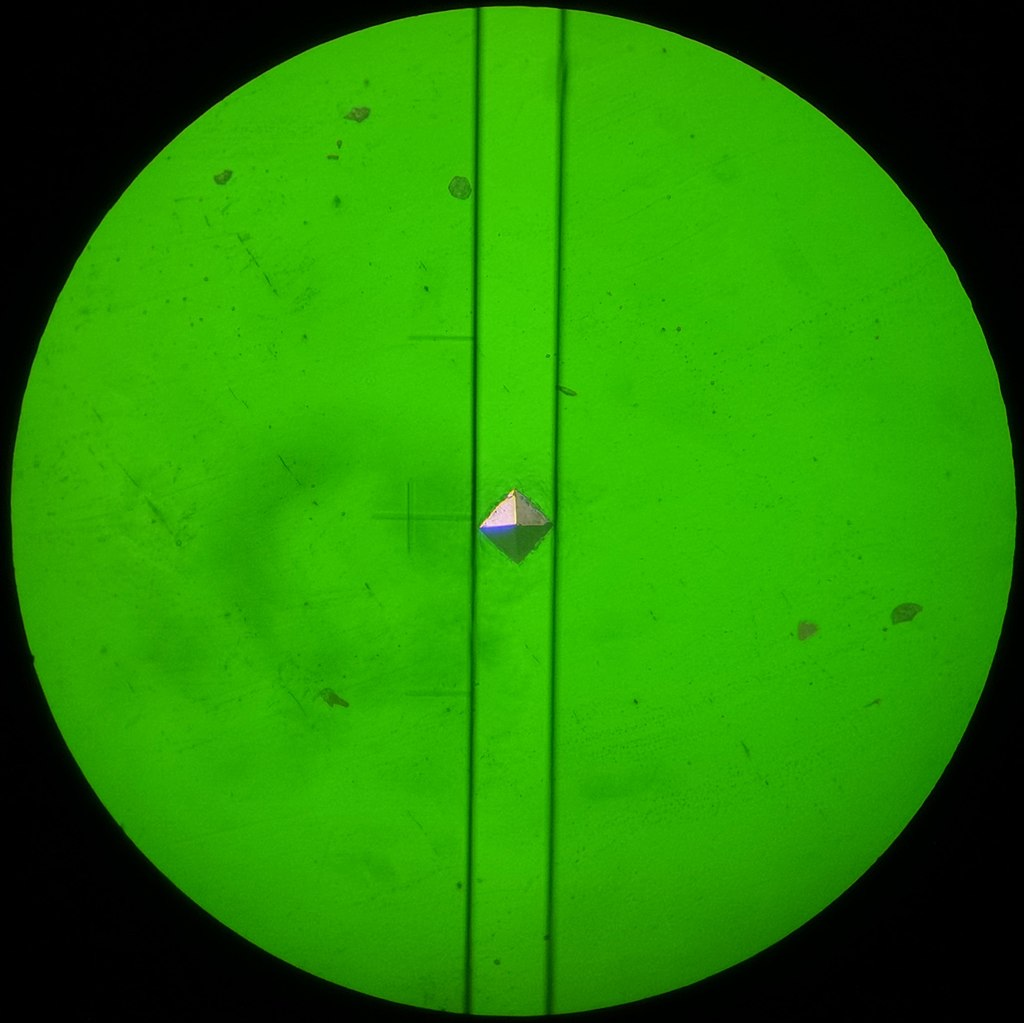
\includegraphics[width=0.8\textwidth]{images/1024px-Vicker_Hardness_-_Diamond_Indentation.jpg}
    \caption{Illustration showing the diamond-shaped indenter and the parallel lines used for measuring the indentation. (Wikipedia)}
    \label{fig:vickers}
\end{figure}
\end{minipage}\\
\vspace{5pt}
To ensure accuracy and consistency, the indentation was measured twice for the alloy. This procedure was repeated for all three alloys, and the resulting hardness values were recorded on an A4 sheet (see Figure \ref{fig:alloys}) for later analysis.\\[8pt]
Although the machine automatically calculates the hardness, it is important to understand the underlying process. The diagonals of the indentation $d_1$ and $d_2$ are used to calculate the Vickers hardness by determining the surface area of the indent. This area depends on the average of the two diagonal measurements, $d_1$ and $d_2$, as well as the geometry of the indentation. Together, these provide the necessary data to compute the material's hardness.\\[8pt]
Here, I demonstrate and derive the pertinent equation and calculation for the HV5 test:
\begin{figure}[H]
    \centering
    \begin{minipage}{0.45\textwidth}\centering
        \vspace{1em}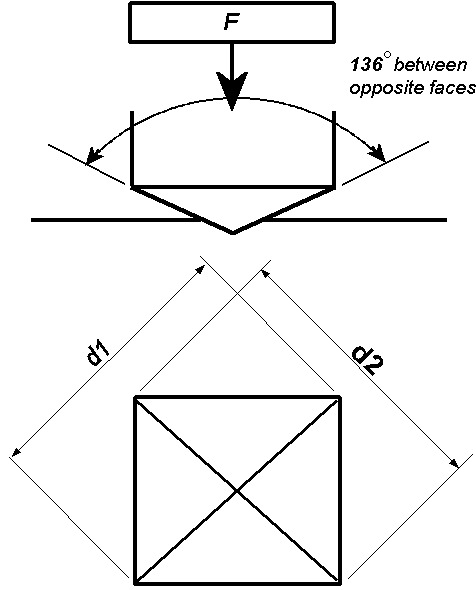
\includegraphics[width=0.8\textwidth]{figures/3537580_orig-0000.jpg}
        \caption{Diagram showing the diamond-shaped indenter with the 136° angle and diagonals \(d_1\) and \(d_2\).}
        \label{fig:vickers-diagram}
    \end{minipage}\hfill
    \begin{minipage}{0.51\textwidth}
        The Vickers hardness (HV) is calculated using the applied force (\(F\)) and the surface area (\(A\)) of the indentation. 
        \begin{equation}
            \text{HV} = \frac{F}{A}
        \end{equation}
        \begin{itemize}[itemsep=-1mm]
            \item HV: Vickers hardness (dimensionless)
            \item \(F\): Applied force (kgf or N)
            \item \(A\): Surface area of the indentation (mm\(^2\))
            
        \end{itemize}
        The formula for $A$ incorporates the geometry of the diamond pyramid indenter, 
        Such that surface area \(A\) can be expressed as:
        \begin{equation}
            A = \frac{d^2}{2\sin\left(\frac{136^\circ}{2}\right)} \approx \frac{d^2}{1.854} 
        \end{equation}
        Where:  
        \begin{itemize}[itemsep=-1mm]
            \item \(A\): Surface area of the indentation (mm\(^2\))
            \item \(d\): Arithmetic mean of the diagonals \(d_1\) and \(d_2\) (mm)
        \end{itemize}
        in so that it can be rewritten in terms of the diagonals as so:
        \begin{equation}
            A= \frac{\left(\frac{d_1+d_2}{2}\right)^2}{2\sin\left(\frac{136^\circ}{2}\right)} \approx \frac{\left(d_1 + d_2\right)^2}{7.236}
        \end{equation}
    \end{minipage}\\
\end{figure}
\vspace{-0.1em}\noindent
Thus the derived formula is commonly shown as
\begin{equation}
    {\text{HV} = \frac{F}{A} \approx \, \frac{1.854 \times F}{d^2} \approx \, \frac{7.236\times F}{\left(d_1 + d_2\right)^2}}    
\end{equation} 
The HV5 test we conducted applied a fixed load of 5 kgf (49.03 N), and the hardness was calculated via the machine as:  
\begin{equation}
    \text{HV5} = \frac{49.03}{A} \approx \, \frac{90.902}{d^2} \approx \, \frac{354.781}{\left(d_1 + d_2\right)^2}
\end{equation}
Were values for \(d_1\) and \(d_2\) were determined using the dial on the machine, and the corresponding hardness values are automatically calculated by the machine upon completion. It is important to note that the resulting hardness value is expressed as a dimensionless number.\\The recorded results were documented on the A4 sheet (see Figure \ref{fig:alloys}) and were as follows:
\begin{center}
    \begin{tblr}{
            width=\textwidth,
            colspec={X[3,c]X[0.75,c]X[0.75,c]X[0.75,c]X[0.75,c]X[0.75,c]X[0.75,c]X[0.8,c]X[0.8,c]X[0.8,c]},
            hlines,vlines,
            rows={ht=1\baselineskip},
            row{1} = {ht=1\baselineskip,font=\bfseries,c,m},
            cells={valign=m,halign=c}
        }
        Property (\(\bm{\text{unitless}}\)) & \SetCell[c=2]{c} AR & & \SetCell[c=2]{c} ST & & \SetCell[c=3]{c} PH & & \\
        HV5 (Individual) & 119 & 123 & 36 & 36.8 & 102.8 & 131 & 126 \\
        HV5 (Average) & \SetCell[c=2]{c} 121 & & \SetCell[c=2]{c} 36.4 & & \SetCell[c=3]{c} 118 & & \\
    \end{tblr}
    \caption{HV5 Data}
    \label{tab:hv5}
\end{center}
Here Table \ref{tab:hv5} presents both the individual and average Vickers hardness (HV5) values for each alloy. The individual measurements were recorded, and the averages were calculated using the standard formula \(\frac{\sum x_i}{n}\) to provide representative values.\\[8pt]
A detailed analysis of these results will be provided in the results section, where trends and implications will be thoroughly examined.

\subsection{Tensile Test}
\newpage\vspace*{-5pt}
    \section{Theory}

    \newpage\vspace*{-20pt}
    
    \section{Results}
        \renewcommand{\arraystretch}{1.4}
        \begin{table}[H]
            \centering
            \begin{tblr}{
                    width=\textwidth,
                    colspec={X[0.4,c]X[1,c]X[1.1,c]X[1.9,c]X[1.9,c]X[1.1,c]X[0.8,c]X[0.7,c]},
                    hlines,vlines,
                    cells={valign=m,halign=c}
                }
                \textbf{Nr} & \textbf{Specimen ID} & \textbf{Date} & \textbf{Stress - Maximum Load (N)} & \textbf{Strain Extension at Break (mm)} & \textbf{Thickness (mm)} & \textbf{Width (mm)} & \textbf{CSA \((\text{mm}^2)\)} \\
                1 & ST & 20/11/2024 & 8580 & 19.8 & 1 & 1 & 1.00 \\
                2 & PH & 20/11/2024 & 23800 & 9.8 & 1 & 1 & 1.00 \\
                3 & AR & 20/11/2024 & 24400 & 9.7 & 1 & 1 & 1.00 \\
                \end{tblr}
            \caption{Specimen Data}
            \label{tab:specimen_data}
        \end{table}

    \begin{figure}[H]
        \centering
        \includegraphics[scale=0.56]{figures/graph.png}
        \caption{Machine produced data}
        \label{fig:stress_strain}
    \end{figure}
    
    \newpage\vspace*{-5pt}
    \section{Discussion}

    \newpage\vspace*{-5pt}
    \section{Conclusions}

    \newpage\vspace*{-5pt}
    \section{Recommendations}

    \newpage\vspace*{-5pt}
    \section{References}
    \begin{enumerate}
        \item Eurotherm (2024) \textit{An Introduction to the Heat Treatment of Metallic Alloys}. Available at: \url{https://www.eurotherm.com/sv/heat-treatment-articles-sv/an-introduction-to-the-heat-treatment-of-metallic-alloys/} [Accessed 19 December 2024].
        
        \item Rajaa, S. M., Abdulhadi, H. A., Jabur, K. S., and Mohammed, G. R. (2018). Aging Time Effects on the Mechanical Properties of Al 6061-T6 Alloy. Available at: \url{https://pdfs.semanticscholar.org/a99b/8b7e771be0fecaaeb970074c7a2871a77032.pdf} [Accessed 19 December 2024].        

        \item Singh, P., Singh, R.K. \& Das, A.K. (2023) \textit{‘Optimization of Heat Treatment Cycle for Cast-Al6082 Alloy to Enhance the Mechanical Properties’}. Research Square. Available at: \url{https://assets-eu.researchsquare.com/files/rs-3363991/v1/9cd60f8c-a164-4e04-8552-1933478eaded.pdf?c=1711467707} [Accessed 7 December 2024].
        
        \item Thyssenkrupp Materials (2023) \textit{Aerospace Grade Aluminium}. Available at: \url{https://www.thyssenkrupp-materials.co.uk/aerospace-grade-aluminum} [Accessed 19 December 2024].
        
        \item Truventor (2019) \textit{Aluminium 6082 Data Sheet}. Available at: \url{https://truventor.ai/assets/pdf/datasheets/Aluminium%206082.pdf} [Accessed 19 December 2024].
        
        \item Rovida, C., Alépée, N., Api, A.M., Basketter, D.A., Bois, F.Y., Caloni, F., Corsini, E., Daneshian, M., Eskes, C., Ezendam, J., Fuchs, H., Hayden, P., Hegele-Hartung, C., Hoffmann, S., Hubesch, B., Jacobs, M.N., Jaworska, J., Kleensang, A., Kleinstreuer, N., Lalko, J., Landsiedel, R., Lebreux, F., Luechtefeld, T., Locatelli, M., Mehling, A., Natsch, A., Pitchford, J.W., Prater, D., Prieto, P., Schepky, A., Schüürmann, G., Smirnova, L., Toole, C., van Vliet, E., Weisensee, D. and Hartung, T. (2015) \textit{Integrated Testing Strategies (ITS) for Safety Assessment}. Available at: \url{https://www.researchgate.net/publication/6538912_The_Principles_of_Weight_of_Evidence_Validation_of_Test_Methods_and_Testing_Strategies_The_Report_and_Recommendations_of_ECVAM_Workshop_58} [Accessed 20 December 2024].
        
        \item Alan Turing Institute (2024) \textit{Data-Driven Experiment Design}. Available at: \url{https://www.turing.ac.uk/research/research-projects/data-driven-experiment-design} [Accessed 20 December 2024].
        
    \end{enumerate}

    
    
    %https://nasruldesign.weebly.com/ndt---brief-overview.html
    %https://www.sciencedirect.com/topics/materials-science/indentation-hardness-testing
    %https://nasruldesign.weebly.com/uploads/7/4/1/9/7419180/hardness_testing_manual.pdf
    

    \newpage\vspace*{-5pt}
    
   
    
\section{Appendix}
\normalsize
\renewcommand{\thesubsection}{\Alph{subsection}}

\subsection{BHN (Brinell Hardness Number)}
The Brinell Hardness Number (BHN) measures a material's resistance to deformation, determined by the indentation left by a hard steel or carbide ball pressed into the material under a specified load. This test is commonly used for materials with a coarse or heterogeneous grain structure.\\[1em]
The formula for calculating the Brinell Hardness Number is:
\begin{equation}
    BHN = \frac{2P}{\pi D (D - \sqrt{D^2 - d^2})}
\end{equation}
Where:
\begin{itemize}[itemsep=-1mm]
    \item \( P \) : applied load in kilogram-force (kgf),
    \item \( D \) : diameter of the indenter (typically 10 mm),
    \item \( d \) : diameter of the indentation (mm).
\end{itemize}
\textbf{Note}: The Brinell test may use either $P$ or $F$ for the load, depending on the source.\\ 
The BHN provides insight into a material's ability to resist wear and deformation, which is important for assessing the durability and suitability of metals in various engineering applications. BHN values are particularly useful for testing larger, rougher materials and are commonly applied to metals like steel and cast iron. The results help predict wear resistance and strength under load.


\subsection{RSM and FFS}
\textbf{Response Surface Methodology (RSM)} is a type of adaptive or sequential design. Sequential designs involve multiple rounds of experimentation, with the choice of treatments in each later round being dependent on the data accumulated from completed rounds. RSM is usually used to identify some sort of optimum, often for industrial production. Sequential designs also exist outside of the RSM framework, however, such as Bayesian Adaptive Experimental Design.\\[8pt]
\textbf{Fractional Factorial Designs (FFDs)} are a specific group of experimental designs. They allow useful information to be extracted from relatively tiny experiments, especially in situations with a large number of predictors. The central (quite reasonable) assumption is that higher-order interactions are less important than lower-order ones and main effects, which is called the "sparsity-of-effects principle". Experimental designs can therefore be scaled down by neglecting the higher-order interactions. This scaling down involves intentionally confounding (‘aliasing’) combinations of factors relative to the full factorial experiment, with the consequence that one cannot estimate each separate main effect and interaction term. We can still learn a great deal of useful information from the data despite this limitation, though.\\[8pt]
\textbf{How RSM and FFDs interact:}\\[8pt]
FFDs are most often used as a component of RSM. But they can in principle be used independently, either as part of a one-shot experiment, or as part of a sequential design approach that does not involve RSM. They seem unlikely to be very useful when used in a one-shot experiment, which is probably why they are so tightly connected to RSM.\\[8pt]
Additionally, RSM can take as its input experimental designs that are not FFDs. Central Composite Designs and Box-Behnken designs are two other commonly-used designs.\\[8pt]
My thanks to kjetil b halvorsen and Gregg H for their input and the suggested resources. I was not able to lay my hands on the Montgomery book but found the Box, Hunter \& Hunter book very useful.

\end{document}
